% \documentclass[conference, review]{IEEEtran}
% \documentclass[sigconf,authordraft]{acmart}
% \documentclass[conference]{IEEEtran}
\documentclass[sigconf]{acmart}
% \documentclass[sigconf]{acmart}
% \IEEEoverridecommandlockouts
% The preceding line is only needed to identify funding in the first footnote. If that is unneeded, please comment it out.
% \settopmatter{authorsperrow=3}7-[-7-=]

\usepackage{amsmath,amsfonts}

\usepackage{amsthm}
\usepackage{algorithm}
% \usepackage{algorithmic}
% \usepackage[linesnumbered,ruled,vlined]{algorithm2e}
\usepackage{algpseudocode}

\usepackage{graphicx}
\usepackage{textcomp}
\usepackage{xcolor}
\usepackage{mdframed}
\usepackage{tabularx}
\usepackage{comment}
\usepackage{booktabs}
\usepackage{epsfig}
\usepackage{bm}
\usepackage[tight,footnotesize]{subfigure}
\usepackage{adjustbox}
\usepackage{multirow}
\usepackage{cleveref}

\newcommand{\hl}[1]{\textcolor{red}{#1}}
\newcommand{\kai}[1]{\textcolor{red}{#1}}
\newcommand{\yang}[1]{\textcolor{blue}{#1}}

% \usepackage{mdframed}
% \mdfsetup{
%   linecolor=red,  % Frame color
%   linewidth=2pt,  % Frame line width
% }

\newtheorem{theorem}{Theorem}
\newtheorem{corollary}{Corollary}[theorem]
\newtheorem{lemma}[theorem]{Lemma}



%% Rights management information.  This information is sent to you
%% when you complete the rights form.  These commands have SAMPLE
%% values in them; it is your responsibility as an author to replace
%% the commands and values with those provided to you when you
%% complete the rights form.
% \setcopyright{none}
% \setcopyright{acmcopyright}
% \copyrightyear{2018}
% \acmYear{2018}
% \acmDOI{10.1145/1122445.1122456}
\renewcommand\footnotetextcopyrightpermission[1]{} % Removes footnote with conference information
\settopmatter{printacmref=false}

%% These commands are for a PROCEEDINGS abstract or paper.
\acmConference[Conference acronym 'XX]{Make sure to enter the correct
  conference title from your rights confirmation emai}{June 03--05,
  2018}{Woodstock, NY}
% \acmBooktitle{SC '21: The International ....,
%   June 21--25, 2021, Stockholm, Sweden}
% \acmPrice{15.00}
% \acmISBN{978-1-4503-XXXX-X/18/06}

% \setlength{\floatsep}{0.2em}
% \setlength{\textfloatsep}{1.0em}
% \setlength{\intextsep}{0.2em}
% \setlength{\belowcaptionskip}{0.2em}

%\newcommand{\projectName}{MDZ}

\begin{document}

% \title{IPComp: \underline{I}nterpolation Based \underline{P}rogressive Lossy \underline{Comp}ression for Scientific Applications}
\title{IPComp: \texorpdfstring{\underline{I}}{I}nterpolation Based \texorpdfstring{\underline{P}}{P}rogressive Lossy \texorpdfstring{\underline{Comp}}{Comp}ression for Scientific Applications}

% \title{PSZ: Enhancing the SZ Scientific Lossy Compressor With Progressive Data Retrieval} 

\author{Zhuoxun Yang}
\affiliation{%
  \institution{Florida State University}
  \city{Tallahassee}
  \state{FL}
  \country{USA}}
\email{zy24b@fsu.edu}

\author{Sheng Di}
\affiliation{%
  \institution{The University of Chicago}
  \institution{Argonne National Laboratory}
  \city{Lemont}
  \state{IL}
  \country{USA}}
\email{sdi1@anl.gov}

\author{Longtao Zhang}
\affiliation{%
  \institution{Florida State University}
  \city{Tallahassee}
  \state{FL}
  \country{USA}}
\email{lzhang11@fsu.edu}


\author{Ruoyu Li}
\affiliation{%
  \institution{Florida State University}
  \city{Tallahassee}
  \state{FL}
  \country{USA}}
\email{rl13m@fsu.edu}

\author{Ximiao Li}
\affiliation{%
  \institution{Florida State University}
  \city{Tallahassee}
  \state{FL}
  \country{USA}}
\email{xl24g@fsu.edu}


\author{Jiajun Huang}
\affiliation{%
  \institution{University of California, Riverside}
  \city{Riverside}
  \state{CA}
  \country{USA}}
\email{jhuan380@ucr.edu}


\author{Jinyang Liu}
\affiliation{%
  \institution{University of Houston}
  \city{Houston}
  \state{TX}
  \country{USA}}
\email{jliu217@central.uh.edu}




\author{Franck Cappello}
\affiliation{%
  \institution{The University of Chicago}
  \institution{Argonne National Laboratory}
  \city{Lemont}
  \state{IL}
  \country{USA}}
\email{cappello@mcs.anl.gov}


\author{Kai Zhao}
\authornote{Corresponding author}
\affiliation{%
  \institution{Florida State University}
  \city{Tallahassee}
  \state{FL}
  \country{USA}}
\email{kzhao@cs.fsu.edu}

% \author{\IEEEauthorblockN{
% Kai Zhao\IEEEauthorrefmark{1},
% Sheng Di\IEEEauthorrefmark{2},
% Danny Perez,\IEEEauthorrefmark{3},
% Xin Liang,\IEEEauthorrefmark{4},
% Zizhong Chen\IEEEauthorrefmark{1}, and
% Franck Cappello\IEEEauthorrefmark{2}\IEEEauthorrefmark{5}
% }
% \IEEEauthorblockA{\IEEEauthorrefmark{1}
% %Department of Computer Science \& Engineering\\
% University of California, Riverside, CA, USA}
% \IEEEauthorblockA{\IEEEauthorrefmark{2}
% %Mathematic and Computer Science Division\\
% Argonne National Laboratory, Lemont, IL, USA
% }
% \IEEEauthorblockA{\IEEEauthorrefmark{3}
% Los Alamos National Laboratory, Los Alamos, NM, USA
% }
% \IEEEauthorblockA{\IEEEauthorrefmark{4}
% Missouri University of Science and Technology, Rolla, MO, USA
% }
% \IEEEauthorblockA{\IEEEauthorrefmark{5}
% %Department of Computer Science\\
% University of Illinois at Urbana-Champaign, Champaign, IL, USA}
% kzhao016@ucr.edu, sdi1@anl.gov, 
% danny\_perez@lanl.gov, \\xliang@mst.edu, 
% chen@cs.ucr.edu, cappello@mcs.anl.gov
% \thanks{Corresponding author: Sheng Di, Mathematics and Computer Science Division, Argonne National Laboratory, 9700 Cass Avenue, Lemont, IL 60439, USA}
% }
% \bstctlcite{IEEEexample:BSTcontrol}

% https://vldb.org/pvldb/volumes/18/submission
% https://2025.sigmod.org/calls_papers_sigmod_research.shtml#dates

\begin{abstract}
Compression is a crucial solution for data reduction in modern scientific applications due to the exponential growth of data from simulations, experiments, and observations.
Compression with progressive retrieval capability allows users to quickly access coarse approximations of data and then incrementally refine these approximations to higher fidelity. 
Existing progressive compression solutions suffer from low reduction ratios or high operation costs, effectively undermining the approach's benefits.
In this paper, we propose the first-ever interpolation-based progressive lossy compression solution that has both high reduction ratios and low operation costs. The interpolation-based algorithm has been verified as one of the best for scientific data reduction, but previously, no effort exists to make it support progressive retrieval. Our contributions are three-fold:
(1) We thoroughly analyze the error characteristics of the interpolation algorithm and propose our solution, IPComp, with multi-level bitplane and predictive coding. 
(2) We derive optimized strategies toward minimum data retrieval under different fidelity levels indicated by users through error bounds and bitrates.
(3) We evaluate the proposed solution using six real-world datasets from four diverse domains. Experimental results demonstrate our solution archives up to $487\%$ higher compression ratios and $698\%$ faster speed than other state-of-the-art progressive compressors, and reduces the data volume for retrieval by up to $83\%$ compared to baselines under the same error bound, and reduces the error by up to $99\%$ under the same bitrate.

\end{abstract}

\maketitle  

\section{Introduction}


\begin{figure}[t]
\centering
\includegraphics[width=0.6\columnwidth]{figures/evaluation_desiderata_V5.pdf}
\vspace{-0.5cm}
\caption{\systemName is a platform for conducting realistic evaluations of code LLMs, collecting human preferences of coding models with real users, real tasks, and in realistic environments, aimed at addressing the limitations of existing evaluations.
}
\label{fig:motivation}
\end{figure}

\begin{figure*}[t]
\centering
\includegraphics[width=\textwidth]{figures/system_design_v2.png}
\caption{We introduce \systemName, a VSCode extension to collect human preferences of code directly in a developer's IDE. \systemName enables developers to use code completions from various models. The system comprises a) the interface in the user's IDE which presents paired completions to users (left), b) a sampling strategy that picks model pairs to reduce latency (right, top), and c) a prompting scheme that allows diverse LLMs to perform code completions with high fidelity.
Users can select between the top completion (green box) using \texttt{tab} or the bottom completion (blue box) using \texttt{shift+tab}.}
\label{fig:overview}
\end{figure*}

As model capabilities improve, large language models (LLMs) are increasingly integrated into user environments and workflows.
For example, software developers code with AI in integrated developer environments (IDEs)~\citep{peng2023impact}, doctors rely on notes generated through ambient listening~\citep{oberst2024science}, and lawyers consider case evidence identified by electronic discovery systems~\citep{yang2024beyond}.
Increasing deployment of models in productivity tools demands evaluation that more closely reflects real-world circumstances~\citep{hutchinson2022evaluation, saxon2024benchmarks, kapoor2024ai}.
While newer benchmarks and live platforms incorporate human feedback to capture real-world usage, they almost exclusively focus on evaluating LLMs in chat conversations~\citep{zheng2023judging,dubois2023alpacafarm,chiang2024chatbot, kirk2024the}.
Model evaluation must move beyond chat-based interactions and into specialized user environments.



 

In this work, we focus on evaluating LLM-based coding assistants. 
Despite the popularity of these tools---millions of developers use Github Copilot~\citep{Copilot}---existing
evaluations of the coding capabilities of new models exhibit multiple limitations (Figure~\ref{fig:motivation}, bottom).
Traditional ML benchmarks evaluate LLM capabilities by measuring how well a model can complete static, interview-style coding tasks~\citep{chen2021evaluating,austin2021program,jain2024livecodebench, white2024livebench} and lack \emph{real users}. 
User studies recruit real users to evaluate the effectiveness of LLMs as coding assistants, but are often limited to simple programming tasks as opposed to \emph{real tasks}~\citep{vaithilingam2022expectation,ross2023programmer, mozannar2024realhumaneval}.
Recent efforts to collect human feedback such as Chatbot Arena~\citep{chiang2024chatbot} are still removed from a \emph{realistic environment}, resulting in users and data that deviate from typical software development processes.
We introduce \systemName to address these limitations (Figure~\ref{fig:motivation}, top), and we describe our three main contributions below.


\textbf{We deploy \systemName in-the-wild to collect human preferences on code.} 
\systemName is a Visual Studio Code extension, collecting preferences directly in a developer's IDE within their actual workflow (Figure~\ref{fig:overview}).
\systemName provides developers with code completions, akin to the type of support provided by Github Copilot~\citep{Copilot}. 
Over the past 3 months, \systemName has served over~\completions suggestions from 10 state-of-the-art LLMs, 
gathering \sampleCount~votes from \userCount~users.
To collect user preferences,
\systemName presents a novel interface that shows users paired code completions from two different LLMs, which are determined based on a sampling strategy that aims to 
mitigate latency while preserving coverage across model comparisons.
Additionally, we devise a prompting scheme that allows a diverse set of models to perform code completions with high fidelity.
See Section~\ref{sec:system} and Section~\ref{sec:deployment} for details about system design and deployment respectively.



\textbf{We construct a leaderboard of user preferences and find notable differences from existing static benchmarks and human preference leaderboards.}
In general, we observe that smaller models seem to overperform in static benchmarks compared to our leaderboard, while performance among larger models is mixed (Section~\ref{sec:leaderboard_calculation}).
We attribute these differences to the fact that \systemName is exposed to users and tasks that differ drastically from code evaluations in the past. 
Our data spans 103 programming languages and 24 natural languages as well as a variety of real-world applications and code structures, while static benchmarks tend to focus on a specific programming and natural language and task (e.g. coding competition problems).
Additionally, while all of \systemName interactions contain code contexts and the majority involve infilling tasks, a much smaller fraction of Chatbot Arena's coding tasks contain code context, with infilling tasks appearing even more rarely. 
We analyze our data in depth in Section~\ref{subsec:comparison}.



\textbf{We derive new insights into user preferences of code by analyzing \systemName's diverse and distinct data distribution.}
We compare user preferences across different stratifications of input data (e.g., common versus rare languages) and observe which affect observed preferences most (Section~\ref{sec:analysis}).
For example, while user preferences stay relatively consistent across various programming languages, they differ drastically between different task categories (e.g. frontend/backend versus algorithm design).
We also observe variations in user preference due to different features related to code structure 
(e.g., context length and completion patterns).
We open-source \systemName and release a curated subset of code contexts.
Altogether, our results highlight the necessity of model evaluation in realistic and domain-specific settings.





\section{The \search\ Search Algorithm}
\label{sec:search}

%In traditional ML, structure changes and step (operator) changes are performed before model training, \ie, fixed to the training process, and weights are updated with SGD, because weights are continous, differentiable values, and there are significantly more weights than structure and operator changes. In workflow autotuning, all three types of cogs can be chosen with a unified search-based approach, because all of them are non-differentiable configurations and the number of cogs in different types are all small.
%Thus, \sysname\ only needs to navigate the search space of combination of cogs as the search space to produce its workflow optimization results.

%We propose, \textit{\textbf{\search}}, an adaptive hierarchical search algorithm that autotunes gen-AI workflows based on observed end-to-end workflow results. In each search iteration, \search\ selects a combination of cogs to apply to the workflow and executes the resulting workflow with user-provided training inputs. \search\ evaluates the final generation quality using the user-specified evaluator and measures the execution time and cost for each training input. These results are aggregated and serve as BO observations and pruning criteria.
%the optimizer can condition on and propose better configurations in later trials. The optimizer will also be informed about the violation of any user-specified metric thresholds. More details of this mechanism can be found in Appendix ~\ref{appdx:TPE}.

With our insights in Section~\ref{sec:theory}, we believe that search methods based on Bayesian Optimizer (BO) can work for all types of cogs in gen-AI workflow autotuning because of BO's efficiency in searching discrete search space.
A key challenge in designing a BO-based search is the limited search budgets that need to be used to search a high-dimensional cog space. 
For example, for 4 cogs each with 4 options and a workflow of 3 LLM steps, the search space is $4^{12}$. Suppose each search uses GPT-4o and has 1000 output tokens, the entire space needs around \$168K to go through. A user search budget of \$100 can cover only 0.06\% of the search space. A traditional BO approach cannot find good results with such small budgets.
%The entire search space grows exponentially with the number of cogs and the number of steps in a workflow. Moreover, different cogs and different combinations of cogs can have varying impacts on different workflows. 
%Without prior knowledge, it is difficult to determine the amount of budget to give to each cog.

To confront this challenge, we propose \textit{\textbf{\search}}, an adaptive hierarchical search algorithm that efficiently assigns search budget across cogs based on budget size and observed workflow evaluation results, as defined in Algorithms~\ref{alg:main} and \ref{alg:outer} and described below.
%autotunes gen-AI workflows based on observed end-to-end workflow results.
%\search\ includes a search layer partitioning method, a search budget initial assignment method, an evaluation-guided budget re-allocation mechanism, and a convergence-based early-exiting strategy. We discuss them in details below.

%\zijian{\search\ allows users to specify the optimization budget allowed in terms of the maximum number of search iterations. Based on the relationship between the complexity of the search space and the available budget, we will separate all tunable parameters into different layers each optimized by independent Bayesian optimization routines. Then we will decide the maximum budget each layer can get with a bottom-up partition strategy. Besides search space and resource partition, we also employ a novel allocation algorithm that integrates successive halving~\cite{successivehalving} and a convergence-based early exiting strategy to facilitate efficient usage of assigned budget.}


% The outermost layer searches and selects structures for a workflow; the middle layer searches and selects step options under the workflow structure selected in the outermost layer; the innermost layer searches and selects weights with the given workflow structure and steps. 

\begin{algorithm}[h]
    \caption{\search\ Algorithm}
    \label{alg:main}
      \small
\begin{algorithmic}[1]
\STATE \textbf{Global Value:} $R = \emptyset$ \COMMENT{Global result set}
%\STATE \textbf{Global Value:} $F = \emptyset$ \COMMENT{Global observation set}

%Reduct factor $\eta > 1$, explore width $W$
\STATE \textbf{Input:} User-specified Total Budget $TB$
\STATE \textbf{Input:} Cog set $C = \{c_{11},c_{12},...\}, \{c_{21},c_{22},...\}, \{c_{31},c_{32},...\}$

    \STATE
%\FOR{$i = 1,2,3$}
    %\COMMENT{$\alpha$ is a configurable value default to 1.1}
%\ENDFOR
%\STATE
%    \STATE \{$B_1,B_2,B_3$\} = LayerPartition($C$) \COMMENT{Calculate ideal layer budget}
    %\STATE \textbf{Glob}.budgets = budgets
%    \STATE opt\_layers = init\_opt\_routines() \COMMENT{A list of optimize routine each layer will use for search}
%\STATE
%    \FOR{$i \in L, \dots, 1$}
%        \IF{$i == L$}
 %           \STATE opt\_layers[L] = InnerLayerOpt
  %      \ELSE
   %         \STATE opt\_layers[i] = OuterLayerOpt
            %\STATE opt\_layers[i].next\_layer\_budgets = B[i+1]
            %\STATE opt\_layers[i].next\_layer\_routine = opt\_layers[i+1]
    %    \ENDIF
    %\ENDFOR
%\STATE opt\_layers[1].invoke($\emptyset$, B[1])
\STATE $U = 0$ \COMMENT{Used budget so far, initialize to 0}

\STATE \COMMENT{Perform search with 1 to 3 layers until budget runs out}
\FOR{$L = 1,2,3$} 
        \IF{$L=1$}
            \STATE $C_1 = C_1 \cup C_2 \cup C_3$ \COMMENT{Merge all cogs into a single layer}
        \ENDIF
        \IF{$L==2$}
            \STATE $C_1 = C_1 \cup C_2$ \COMMENT{Merge step and weight cogs}
            \STATE $C_2 = C_3$ \COMMENT{Architecture cog becomes the second layer}
        \ENDIF
        \STATE
    \FOR{$i = 1,..,L$}
    \STATE $NC_i = |C_i|$ \COMMENT{Total number of cogs in layer $L$} 
%    NO_i &= \sum_{L} \{\text{number of possible options in cog } c_{ij}\} \\
    \STATE $S_i = NC_i^\alpha$ \COMMENT{Estimated expected search size in layer $i$}
    \ENDFOR
    \STATE $E_L = \prod\limits_{i=1}^{L}S_i$ \COMMENT{Expected total search size in the current round}
    \STATE $E = TB - U > E_L$ ? $E_L$ : $(TB - U)$ \COMMENT{Consider insufficient budget} 
    \IF{$L==3$ and $(TB - U)$ > $E_L$}
         \STATE $E = TB - U$ \COMMENT{Spend all remaining budget if at 3 layer}
    \ENDIF
    %\STATE$TL = |N|$ \COMMENT{number of layers}
    \FOR{$i = 1,..,L$}
        \STATE $B_i =  \lfloor S_i \times \sqrt[L]{\frac{E}{E_L}}\rfloor$
        %$B$ = BudgetAssign($N$, $TL$, $TB$)
        \COMMENT{Assign budget proportionally to $S_i$}
    \ENDFOR
    \STATE
\STATE \texttt{LayerSearch} ($\emptyset$, $B$, $L$, $B_L$) \COMMENT{Hierarchical search from layer $L$}
\STATE
\STATE $U = U + E$
\IF{$U \geq TB$}
\STATE break \COMMENT{Stop search when using up all user budget}
\ENDIF
\ENDFOR
%\STATE
%\STATE $O$ = \texttt{SelectBestConfigs} ($R$)
%\IF{$L == 1$}
%    \STATE InnerLayerOpt($\emptyset$, B[1])
%\ELSE
%    \STATE OuterLayerOpt($\emptyset$, B[1], 1)
%\ENDIF
\STATE
\STATE \textbf{Output:} $O$ = \texttt{SelectBestConfigs} ($R$) \COMMENT{Return best optimizations}
\end{algorithmic}
\end{algorithm}

\subsection{Hierarchical Layer and Budget Partition}
\label{sec:ssp}

%We motivate \search's adaptive hierarchical search 
A non-hierarchical search has all cog options in a single-layer search space for an optimizer like BO to search, an approach taken by prior workflow optimizers~\cite{dspy-2-2024,gptswarm}.
With small budgets, a single-layer hierarchy allows BO-like search to spend the budget on dimensions that could potentially generate some improvements.
%While given enough budget, the single-layer space can be extensively searched to find global optimal, with little budget, 
However, a major issue with a single-layer search space is that a search algorithm like BO can be stuck at a local optimum even when budgets increase.
% (unless the budget is close to covering a very large space across dimensions).
To mitigate this issue, our idea is to perform a hierarchical search that works by choosing configurations in the outermost layer first, then under each chosen configuration, choosing the next layer's configurations until the innermost layer. 
With such a hierarchy, a search algorithm could force each layer to sample some values. Given enough budget, each dimension will receive some sampling points, allowing better coverage in the entire search space. However, with high dimensionality (\ie, many types of cogs) and insufficient budget, a hierarchical search may not be able to perform enough local search to find any good optimizations.

To support different user-specified budgets and to get the best of both approaches, we propose an adaptive hierarchical search approach, as shown in Algorithm~\ref{alg:main}.
\search\ starts the search by combining all cogs into one layer ($L=1$, line 9 in Algorithm~\ref{alg:main}) and estimating the expected search budget of this single layer to be the total number of cogs to the power of $\alpha$ (lines 16-19, by default $\alpha = 1.1$). This budget is then passed to the \texttt{LayerSearch} function (Algorithm~\ref{alg:outer}) to perform the actual cog search. When the user-defined budget is no larger than this estimated budget, we expect the single-layer, non-hierarchical search to work better than hierarchical search.
%as the budget for this single layer.

If the user-defined budget is larger, \search\ continues the search with two layers ($L=2$), combining step and weight cogs into the inner layer and architecture cogs as the outer layer (lines 11-14).
\search\ estimates the total search budget for this round as the product of the number of cogs in each of the two layers to the power of $\alpha$ (lines 16-20). It then distributes the estimated search budget between the two layers proportionally to each layer's complexity (lines 22-24) and calls the upper layer's \texttt{LayerSearch} function. Afterward, if there is still budget left, \search\ performs a last round of search using three layers and the remaining budget in a similar way as described above but with three separate layers (architecture as the outermost, step as the middle, and weight cogs as the innermost layer). Two or three layers work better for larger user-defined budgets, as they allow for a larger coverage of the high-dimensional search space.

Finally, \search\ combines all the search results to select the best configurations based on user-defined metrics (line 34).

%\search\ organizes cogs by having architecture cogs in the outer-most search layer, step cogs in the middle layer, and weight cogs in the inner-most layer (line 4 in Algorithm~\ref{alg:main}).
%This is because step cogs' input and output format are dependent on the workflow structure, and the effectiveness of weights (\eg, prompting) are dependent on steps (\eg, LLM model). 

% increases the number of layers until hitting the user-specified total search budget, $TB$

%Thus, the first step of \search\ is to determine the number of layers in its hierarchy and what cogs to include in a layer.
%Intuitively, structure cogs should be placed in the outer-most search layer to be determined first before exploring other cogs. This is because other cogs change node and edge values, and it is easier for 
%However, instead of a fixed number of layers in the hierarchy, we adapt the cog layering according to user-specified total search budgets, $TB$, and the complexity of each layer, using Algorithm~\ref{alg:main}.

% the following \texttt{LayerPartition} method.
%We begin by modeling the relationship between the expected number of evaluations and the number of cogs as well as the number of options in each layer:

%We first consider the identity of each cog in the search space. All structure-cogs will be placed in the outer-most search layer exclusively, which is similar to non-differentiable NAS in traditional ML training. This layer will fix the workflow graph and pass it to the following layer, allowing a stabilized search space for faster convergence.

%Since step-cogs will not create a changing search space, the partition of step-cogs and weight-cogs is conditioned on the search space complexity and the given total budget. Separating step-cogs out can benefit from a more flexible budget allocation strategy and broader exploration for local search at weight-cogs but performs poorly when the given budget is more constrained, in that case, we will optimize them jointly in the same layer.


%\small
%\begin{align*}
%    C &= \{c_{11},c_{12},...\}, \{c_{21},c_{22},...\}, \{c_{31},c_{32},...\} \\
%    NC_i &= \text{total number of cogs in layer i} \\
%    NO_i &= \sum_{j} \{\text{number of possible options in cog } c_{ij}\} \\
%    N_i &= max(NC_i^\alpha,NO_i) \\
%    N_i &= \sum_{j} \{\text{number of possible options in } C_{ij}\} \\
%    N_i &= max(|C_i|^\alpha, N_i) \\
%    B_j &= \prod\limits_{i=1}^{j}N_i, j \in \{1,2,3\}
%\end{align*}

%\normalsize
%where $L$ represents the total number of layers and can be 1, 2, or 3. 
%$C$ represents the entire cog search space, with each row $c_{i*}$ being one of the three types of cogs and lower layers having lower-numbered rows (\eg, $c_{1*}$ being weight cogs). $NC_i$ is the number of cogs in layer $i$, and $NO_i$ is the total number of options across all cogs in layer $i$. $N_i$ is our estimation of the complexity of layer $i$ based on $NC_i$ and $NO_i$ ($\alpha$ is a configurable weight to control the importance between $NC_i$ and $NO_i$; by default $\alpha = 1.1$). 
%$\alpha$ stands for a control parameter, setting the intensity of this scaling behavior w.r.t the number of cogs, we found that $\alpha = 1.2$ is empirically sufficient and efficient for optimizing real workloads. 
%$B_j$ is the expected total number of workflow evaluations for all the lower $j$ layers.
%After calculating $B_1$, $B_2$, and $B_3$, we compare the total budget $TB$ with them.
%When $TB \geq B_3$, we set the total number of layers, $TL$, to 3. When $B_2 \leq TB < B_3$, we set the total number of layers to 2 and merge the step and weight cogs into one layer. When $TB < B_1$, we put all cogs in one layer.
%We only create a separate layer for step-cogs when the given budget $TB$ is greater or equal to the total expected budget for three layers.

%\subsection{Seach Budget Partition}
%\label{sec:sbp}
%After determining cog layers, we distribute the total budget, $TB$, across the layers proportionally to each layer's expected budget $N_i$: , which is the \texttt{BudgetAssign} function.
%We follow a bottom-up partition strategy, where lower layers will try to greedily take the expected budget. This stems from two simple heuristics: (1) feedback to the upper layer is more accurate when the succeeding layer is trained with enough iterations, and (2) the effectiveness of a structure change depends on the setting of individual steps in the workflow (\eg, majority voting is more powerful when each LLM-agent is embedded with diverse few-shot examples or reasoning styles). In cases where the given resource exceeds the total expected budget, 
%We assign $TB$ across layers proportionally to their expected budget $N_i$. 
%The budget assigned at each layer $B_i$ given the total available number of evaluations $TB$ is obtained as follows:

%\small
%\begin{align}
%B_i &=  \lfloor N_i \times \sqrt[L]{\frac{TB}{B^*}}\rfloor
%    B_L &= \begin{cases}
%        min(N_L, TB) & TB < B^* \\
%        \lfloor N_L \times \sqrt[L]{\frac{TB}{B^*}}\rfloor & TB \geq B^*
%    \end{cases}
%    \\
%    B_i &= \begin{cases}
%        min(N_i, \lfloor\frac{TB}{\prod_{j=i+1}^L B_j}\rfloor) & TB < B^* \\
%        \lfloor N_i \times \sqrt[L]{\frac{TB}{B^*}}\rfloor & TB \geq B^*
%    \end{cases}
%\end{align}

%\normalsize


\subsection{Recursive Layer-Wise Search Algorithm}
%The calculation above pre-assigns cogs to layers and search budgets to each layer. 
We now introduce how \search\ performs the actual search in a recursive manner until the inner-most layer is searched, as presented in Algorithm~\ref{alg:outer} \texttt{LayerSearch}. 
Our overall goal is to ensure strong cog option coverage within each layer while quickly directing budgets to more promising cog options based on evaluation results.
%So far, we have determined the optimization layer structure and the maximum allowed search iteration each layer will get. Next, we introduce how the budget is consumed in each layer. The inner-most layer, where weight-cogs, and potentially step-cogs, reside, follows the conventional Bayesian optimization process, exhausting all budgets unless an early stop signal is sent. This signal will be triggered when the current optimizer witnesses $p$ consecutive iterations without any improvements above the threshold. All optimization layers use early stopping to avoid budget waste.
%Algorithm~\ref{alg:inner} describes the search happening at the inner-most (bottom) layer, and 
Specifically, every layer's search is under a chosen set of cog configurations from its upper layers ($C_{chosen}$) and is given a budget $b$. 
In the inner-most layer (lines 7-20), \search\ samples $b$ configurations and evaluates the workflow for each of them together with the configurations from all upper layers ($C_{chosen}$). The evaluation results are added to the feedback set $F$ as the return of this layer.

\begin{algorithm}[h]
  %\algsetup{linenosize=\tiny}
  \small
    \caption{\texttt{LayerSearch} Function}
    \label{alg:outer}
\begin{algorithmic}[1]
%\STATE \textbf{Global Config:} Reduct factor $\eta > 1$, explore width $W$
\STATE \textbf{Global Value:} $R$ \COMMENT{Global result set}
%\STATE \textbf{Global Value:} $F$ \COMMENT{Global observation set}
\STATE \textbf{Input:} $C_{chosen}$: configs chosen in upper layers
\STATE \textbf{Input:} $B$: Array storing assigned budgets to different layers
\STATE \textbf{Input:} $curr\_layer$: this layer's level
\STATE \textbf{Input:} $curr\_b$: this layer's assigned budget
%\STATE
%\FUNCTION{LayerSearch\hspace{0.4em}($C_{chosen}$, $B$, $curr\_layer$, $curr\_b$)}

    \STATE
    \STATE \COMMENT{Search for inner-most layer}
    \IF{curr\_layer == 1}
        \STATE $F = \emptyset$ \COMMENT{Init this layer's feedback set to empty}
        %\STATE $F^{\prime} = match(C_{chosen}, F)$ \COMMENT{Local feedback set}
        \FOR{$k = 0, \dots, curr\_b$}
            \STATE $\lambda$ = \texttt{TPESample} (1) \COMMENT{Sample one configuration using TPE}
            \STATE $f = $ \texttt{EvaluateWorkflow} ($C_{chosen} \cup \lambda$)
            \STATE $R = R \cup \{C_{chosen} \cup \lambda\}$ \COMMENT{Add configuration to global $R$}
            \IF{\texttt{EarlyStop} (f)}
            \STATE break
            \ENDIF
            \STATE $F = F \cup \{f\}$ \COMMENT{Add evaluate result to feedback $F$}
        \ENDFOR
        %\STATE $F = F \cup F^{\prime}$
        \STATE \textbf{Return} $F$
    \ENDIF
    \STATE
    \STATE \COMMENT{Search for non-inner-most layer}
    %\STATE $K = \lfloor \frac{b}{W} \rfloor$, 
    \STATE $b\_used = 0$, $TF = \emptyset$ \COMMENT{Init this layer's used budget and feedback set}
    \STATE $R = \lceil\frac{curr\_b}{\eta}\rceil$, $S = \lfloor\frac{curr\_b}{R}\rfloor$ \COMMENT{Set $R$ and $S$ based on $curr\_b$}
    \STATE
    \WHILE{$b\_{used}$ $\leq$ $curr\_b$}
        \STATE \COMMENT{Sample $W$ configs at a time until running out of $curr\_b$}
        \STATE $n = (curr\_b - b_{used})$ > $W$ ? $W$ : $(curr\_b - b_{used})$
        %\IF{$b - b_{used} < W$}
        %    \STATE $n = b_l - b_{used}$
        %\ELSE
         %   \STATE $n=W$
        %\ENDIF
        \STATE $b\_used$ += $n$
        %\STATE $n = \text{min}(W,\ b_l - kW)$ \COMMENT{Propose $W$ configs and meet $b_l$ constraint}
        \STATE $\Theta = $ \texttt{TPESample} ($n$) \COMMENT{Sample a chunk of $n$ configs in the layer} 
        %\STATE $F^{\prime} = match(C_{chosen}, F)$ \COMMENT{Per-chunk feedback set}
        \STATE $F = \emptyset$ \COMMENT{Init this layer's feedback set to empty}
        \STATE
        \FOR{$s = 0, 1, \dots, S$}
            \STATE $r_s = R\cdot \eta^s$
            \FOR{$\theta \in \Theta$}
                %\IF{$curr\_layer < max\_layer$}
                    \STATE $f =$ \texttt{LayerSearch} ($C_{chosen} \cup \{\theta\}$, $B$, curr\_layer$-1$, $r_s$)
                %\ELSE
                %    \STATE $f =$ InnerOpt($\gamma \cup \{\theta\}$, $r_s$)
                %\STATE $f$ = $opt\_layers[current\_layer+1](\gamma \cup \{\theta\}, r_s)$ \{Optimize the current config at the next layer with $r_s$ budget \}
                %\ENDIF
                \STATE $F = F \cup f$ \COMMENT{Add evaluate result to feedback}
                \IF{\texttt{EarlyStop} ($f$)}
                    \STATE $\Theta = \Theta - \{\theta\}$ \COMMENT{Skip converged configs}
                \ENDIF
            \ENDFOR
            \STATE $\Theta$ = Select top $\lfloor \frac{|\Theta|}{\eta}\rfloor$ configs from $F$ based on user-specified metrics
        \ENDFOR
        \STATE
        \IF{\texttt{EarlyStop} ($F$)}
            \STATE break \COMMENT{Skip remaining search if results converged}
        \ENDIF
        \STATE $TF = TF \cup F$
    \ENDWHILE
    %\STATE $F = F \cup TF$
        \STATE \textbf{Return} $TF$

%\ENDFUNCTION

%\STATE \textbf{Output:} Best metrics in all trials
\end{algorithmic}
\end{algorithm}

% consumption\_nextlayer\_bucket = WSR

% for s in 0, 1,...S do
%     w = W*\eta^{s}
%     r = R*\eta^{-s}

% total budget at next layer = b_l / W * WSR = b_l * SR

% b_l * SR <= b_l * B_l+1

% S = B_{l+1} / R



For a non-inner-most layer, \search\ samples a chunk ($W$) of points at a time using the TPE BO algorithm~\cite{bergstra2011tpe} until all this layer's pre-assigned budget is exhausted (lines 27-30). Within a chunk, \search\ uses a successive-halving-like approach to iteratively direct the search budget to more promising configurations within the chunk (the dynamically changing set, $\Theta$). In each iteration, \search\ calls the next-level search function for each sampled configuration in $\Theta$ with a budget of $r_s$ and adds the evaluation observations from lower layers to the feedback set $F$ for later TPE sampling to use (lines 35-37).
In the first iteration ($s=0$), $r_s$ is set to $R\cdot \eta^0=R$ (line 34). After the inner layers use this budget to search, \search\ filters out configurations with lower performance and only keeps the top $\lfloor \frac{|\Theta|}{\eta}\rfloor$ configurations as the new $\Theta$ to explore in the next iteration (line 42). In each next iteration, \search\ increases $r_s$ by $\eta$ times (line 34), essentially giving more search budget to the better configurations from the previous iteration.

The successive halving method effectively distributes the search budget to more promising configurations, while the chunk-based sampling approach allows for evaluation feedback to accumulate quickly so that later rounds of TPE can get more feedback (compared to no chunking and sampling all $b$ configurations at the same time). To further improve the search efficiency, we adopt an {\em early stop} approach where we stop a chunk or a layer's search when we find its latest few searches do not improve workflow results by more than a threshold, indicating convergence (lines 14,38,45).

%algorithm takes as input other cog settings from previous layers and the assigned budget at the current layer. It tiles the search loop into fixed-size blocks (line 4), each runs the SuccessiveHalving (SH) subroutine in the inner loop (line 7-15). In each SH iteration, only top-$1/\eta$-quantile configurations in $\Theta$ will continue in the next round with $\eta$ times larger budget consumption. As a result, exponentially more trials will be performed by more promising configurations. 

%On average, \textit{Outer-layer search} will create $K$ brackets, each granting approximately $WRS$ budget to the next layer. $R$ represents the smallest amount of resource allocated to any configurations in $\Theta$. 

% layer - 1: budget = 4
% K * W <= b\_current layer
% layer -1: itear 0: propose 2

%     SH:
%     2 config -> R
%     1 config -> 2R

%     iteration 1: propose 2 = W
%     SH:
%     2 config -> R
%     1 config -> 2R

% W configs; each has R resource

% W / eta configs; each has R * eta resource

% R -> least resource one config can get = B2 - smth
% R + R*eta + ... + R*eta\^s -> most promising = B2 + smth


% $L2$ is the middle layer where structure-cogs and step-cogs may be placed exclusively. We employ hyperband for its robustness in exploration and exploitation trace-off. If this layer exists, it will instruct $L1$ the number of search iterations to run in each invocation. Specifically, in each iteration at line 4, \sysname will propose $n$ configurations and run SuccessiveHalving (SH) subroutine (line 8-15). SH will optimize each proposal and use the search results from $L1$ to rank their performance. Each time only the top-performing $n \cdot \eta^{-i}$ can continue in the next round with a larger budget. With this strategy, exponentially more search budgets are allocated to more promising configs at $L2$.

% \input{algo-l2-search}

% $L3$ is the outer-most layer for structure-cogs only when $L2$ is created. For this layer, we employ plain SH without hyperband because of its predictable convergence behavior. This is mainly due to two factors: (1) structure change to the workflow is more significant thus different configurations are more likely to deviate after training with the following layers. (2) with the search space partition strategy in Sec ~\ref{sec:ssp}, we can assume the available budget at each layer is substantial when $L3$ exists. Given this prior knowledge, we can avoid grid searching control parameter $n$ as in the hyperband but adopt a more aggressive allocation scheme to bias towards better proposals and moderate search wastes.



%\subsubsection{Runtime Budget Adaptation}
%Using static estimation of the expected budget for each layer is not enough, we also adjust the assignment during the optimization based on real convergence behavior. Specifically, for layer $i$, we record the number of configurations evaluated in each optimize routine. We set the convergence indicator $C_{ij}$ of $j^{th}$ routine with this number if the search early exits before reaching the budget limit, otherwise 2\x of its assigned resource. Then we update $E_i$ with $\frac{\sum_{j}^M C_{ij}}{M}$. \sysname\ will update the budget partition according to Sec~\ref{sec:sbp} for any newly spawned optimizer routines. Besides controlling the proportion of budgets across layers, a smaller/larger $B_{l+1}$ will also guide the SH in Alg~\ref{alg:outer} to shrink/extend the budget $R$ for differentiating config performance.


\section{\sysname\ Design}
\label{sec:cognify}

We build \sysname, an extensible gen-AI workflow autotuning platform based on the \search\ algorithm. The input to \sysname\ is the user-written gen-AI workflow (we currently support LangChain \cite{langchain-repo}, DSPy \cite{khattab2024dspy}, and our own programming model), a user-provided workflow training set, a user-chosen evaluator, and a user-specified total search budget. \sysname\ currently supports three autotuning objectives: generation quality (defined by the user evaluator), total workflow execution cost, and total workflow execution latency. Users can choose one or more of these objectives and set thresholds for them or the remaining metrics (\eg, optimize cost and latency while ensuring quality to be at least 5\% better than the original workflow). 
\sysname\ uses the \search\ algorithm to search through the cog space.
When given multiple optimization objectives, \sysname\ maintains a sorted optimization queue for each objective and performs its pruning and final result selection from all the sorted queues (possibly with different weighted numbers).
To speed up the search process, we employ parallel execution, where a user-configurable number of optimizers, each taking a chunk of search load, work together in parallel. %Below, we introduce each type of cogs in more details.
\sysname\ returns multiple autotuned workflow versions based on user-specified objectives.
\sysname\ also allows users to continue the auto-tuning from a previous optimization result with more budgets so that users can gradually increase their search budget without prior knowledge of what budget is sufficient.
Appendix~\ref{sec:apdx-example} shows an example of \sysname-tuned workflow outputs. 
\sysname\ currently supports six cogs in three categories, as discussed below. 

%In \sysname, we call every workflow optimization technique a {\em cog}, including structure-changing cogs like task decomposition, step-changing cogs like model selection, and weight-changing cogs like adding few-shot examples to prompts. 
%\sysname\ places structure-changing cogs in the outermost layer, step cogs in the middle layer, and weight cogs in the innermost layer, because \fixme{TODO}.


\subsection{Architecture Cogs}
\label{sec:structure-cog}
%Changing the structure of a workflow can potentially improve its generation quality (\eg, by using multiple steps to attempt at a task in parallel or in chain) or reduce its execution cost and latency (\eg, by merging or removing steps).
\sysname\ currently supports two architecture cogs: task decomposition and task ensemble.
Task decomposition~\cite{khot2023decomposed} breaks a workflow step into multiple sub-steps and can potentially improve generation quality and lower execution costs, as decomposed tasks are easier to solve even with a small (cheaper) model.
There are numerous ways to perform task decomposition in a workflow. 
%, as all LM steps can potentially be decomposed and into different numbers of sub-steps in different ways. Throwing all options to the Bayesian Optimizer would drastically increase the search space for \sysname. 
To reduce the search space, we propose several ways to narrow down task decomposition options. Even though we present these techniques in the setting of task decomposition, they generalize to many other structure-changing tuning techniques.

%First, we narrow down a selected set of steps in a workflow to decompose. 
Intuitively, complex tasks are the hardest to solve and worth decomposition the most. We use a combination of LLM-as-a-judge \cite{vicuna_share_gpt} and static graph (program) analysis to identify complex steps. We instruct an LLM to give a rating of the complexity of each step in a workflow. We then analyze the relationship between steps in a workflow and find the number of out-edges of each step (\ie, the number of subsequent steps getting this step's output). More out-edges imply that a step is likely performing more tasks at the same time and is thus more complex. We multiply the LLM-produced rating and the number of out-edges for each step and pick the modules with scores above a learnable threshold as the target for task decomposition. We then instruct an LLM to propose a decomposition (\ie, generate the submodules and their prompts) for each candidate step. %We provide the LLM with few-shot examples for what proposed modules for a separate task could look like. We also add a refinement step that validates whether the proposition decomposition maintains the semantics of the original trajectory. Once candidate decompositions are generated, those are used for the entirety of the optimization.

{
\begin{figure*}[t!]
\begin{center}
\centerline{\includegraphics[width=0.95\textwidth]{Figures/big_grid.pdf}}
\vspace{-0.1in}
\mycap{Generation Quality vs Cost/Latency.}{Dashed lines show the Pareto frontier (upper left is better). Cost shown as model API dollar cost for every 1000 requests. Cognify selects models
from GPT-4o-mini and Llama-8B. DSPy and Trace do not support model selection and are given GPT-4o-mini for all steps. Trace results for Text-2-SQL and FinRobot have 0 quality and are not included.} 
\Description{Eight graphs with different shapes representing baselines compared to points on a Pareto frontier.}
\label{fig-biggrid}
\end{center}
\end{figure*}
}


The second structure-changing cog that \sysname\ supports is task ensembling. This cog spawns multiple parallel steps (or samplers) for a single step in the original workflow, as well as an aggregator step that returns the best output (or combination of outputs). By introducing parallel steps, \sysname\ can optimize these independently with step and weight cogs. This provides the aggregator with a diverse set of outputs to choose from. 
%The aggregator is prompted with the role of the samplers, as well as the inputs to each. It also receives a criteria by which it should make a decision. We choose to prompt it with a qualitative description of how it should resolve discrepancies between outputs. 


\subsection{Step Cogs}
We currently support two step-changing cogs: model selection for language-model (LM) steps and code rewriting for code steps.

For model selection, to reduce its search space, we identify ``important'' LM steps---steps that most critically impact the final workflow output to reduce the set \search\ performs TPE sampling on. Our approach is to test each step in isolation by freezing other steps with the cheapest model and trying different models on the step under testing. 
We then calculate the difference between the model yielding the best and worst workflow results as the importance of the step under testing. %For each model, we get the workflow output quality score using sampled user-supplied inputs and user-specific evaluator. We then calculate the difference between the highest and lowest scores as this module's importance. 
After testing all the steps, we choose the steps with the highest K\% importance as the ones for TPE to sample from.
%, where K is determined based on user-chosen stop criteria. We then initialize the Bayesian optimization to start with the state where important modules use the largest model and all other modules use the cheapest model. We set the TPE optimization bandwidth of each module to be the inverse of importance, \ie, the more important a module is the more TPE spends on optimizing.

The second step cog \sysname\ supports is code rewriting, where it automatically changes code steps to use better implementation. To rewrite a code step, \sysname\ finds the $k$ worst- and best-performing training data points and feeds their corresponding input and output pairs of this code step to an LLM. We let the LLM propose $n$ new candidate code pieces for the step at a time.
%in parallel to generate a set of $n$ candidates.
In subsequent trials, the optimizer dynamically updates the candidate set using feedback from the evaluator.


\subsection{Weight Cogs}
\sysname\ currently supports two weight-changing cogs: reasoning and few-shot examples.
First, \sysname\ supports adding reasoning capability to the user's original prompt, with two options: zero-shot Chain-of-Thought \cite{wei2022chain} (\ie, ``think step-by-step...'') and dynamic planning \cite{huang2022language} (\ie, ``break down the task into simpler sub-tasks...''). These prompts are appended to the user's prompt. In the case where the original module relies on structured output, we support a reason-then-format option that injects reasoning text into the prompt while maintaining the original output schema.

Second, \sysname\ supports dynamically adding few-shot examples to a prompt. At the end of each iteration, we choose the top-$k$-performing examples for an LM step in the training data and use their corresponding input-output pairs of the LM step as the few-shot examples to be appended to the original prompt to the LM step for later iterations' TPE sampling. As such, the set of few-shot examples is constantly evolving during the optimization process based on the workflow's evaluation results. 
%Few-shot examples are available to all modules, even intermediate steps in the workflow. We use the full trajectory of each request to generate examples for the intermediate steps. Furthermore, we automatically filter out examples that do not meet a user-specified threshold. 



\definecolor{darkgreen}{rgb}{0.0, 0.5, 0.0}
\definecolor{violet}{rgb}{0.56, 0.0, 1.0}
\section{Evaluation}
We apply our methodology to derive counterfactual policies for various MDPs, addressing three main research questions: (1) how does our policy's performance compare to the Gumbel-max SCM approach; (2) how do the counterfactual stability and monotonicity assumptions impact the probability bounds; and (3) how fast is our approach compared with the Gumbel-max SCM method?

\begin{figure*}
    \centering
    %
    \resizebox{0.6\textwidth}{!}{
        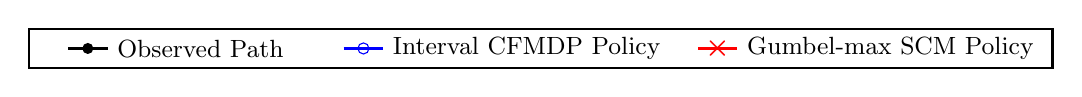
\begin{tikzpicture}[scale=1.0, every node/.style={scale=1.0}]
            \draw[thick, black] (-3, -0.25) rectangle (10, 0.25);
            %
            \draw[black, line width=1pt] (-2.5, 0.0) -- (-2,0.0);
            \fill[black] (-2.25,0.0) circle (2pt); %
            \node[right] at (-2,0.0) {\small Observed Path};
            
            %
            \draw[blue, line width=1pt] (1.0,0.0) -- (1.5,0.0);
            \node[draw=blue, circle, minimum size=4pt, inner sep=0pt] at (1.25,0.0) {}; %
            \node[right] at (1.5,0.0) {\small Interval CFMDP Policy};
            
            %
            \draw[red, line width=1pt] (5.5,0) -- (6,0);
            \node[red] at (5.75,0) {$\boldsymbol{\times}$}; %
            \node[right] at (6,0) {\small Gumbel-max SCM Policy};
        \end{tikzpicture}
    }\\
    %
    \subfigure[\footnotesize Lowest cumulative reward: Interval CFMDP ($312$), Gumbel-max SCM ($312$)]{%
        \resizebox{0.76\columnwidth}{!}{
             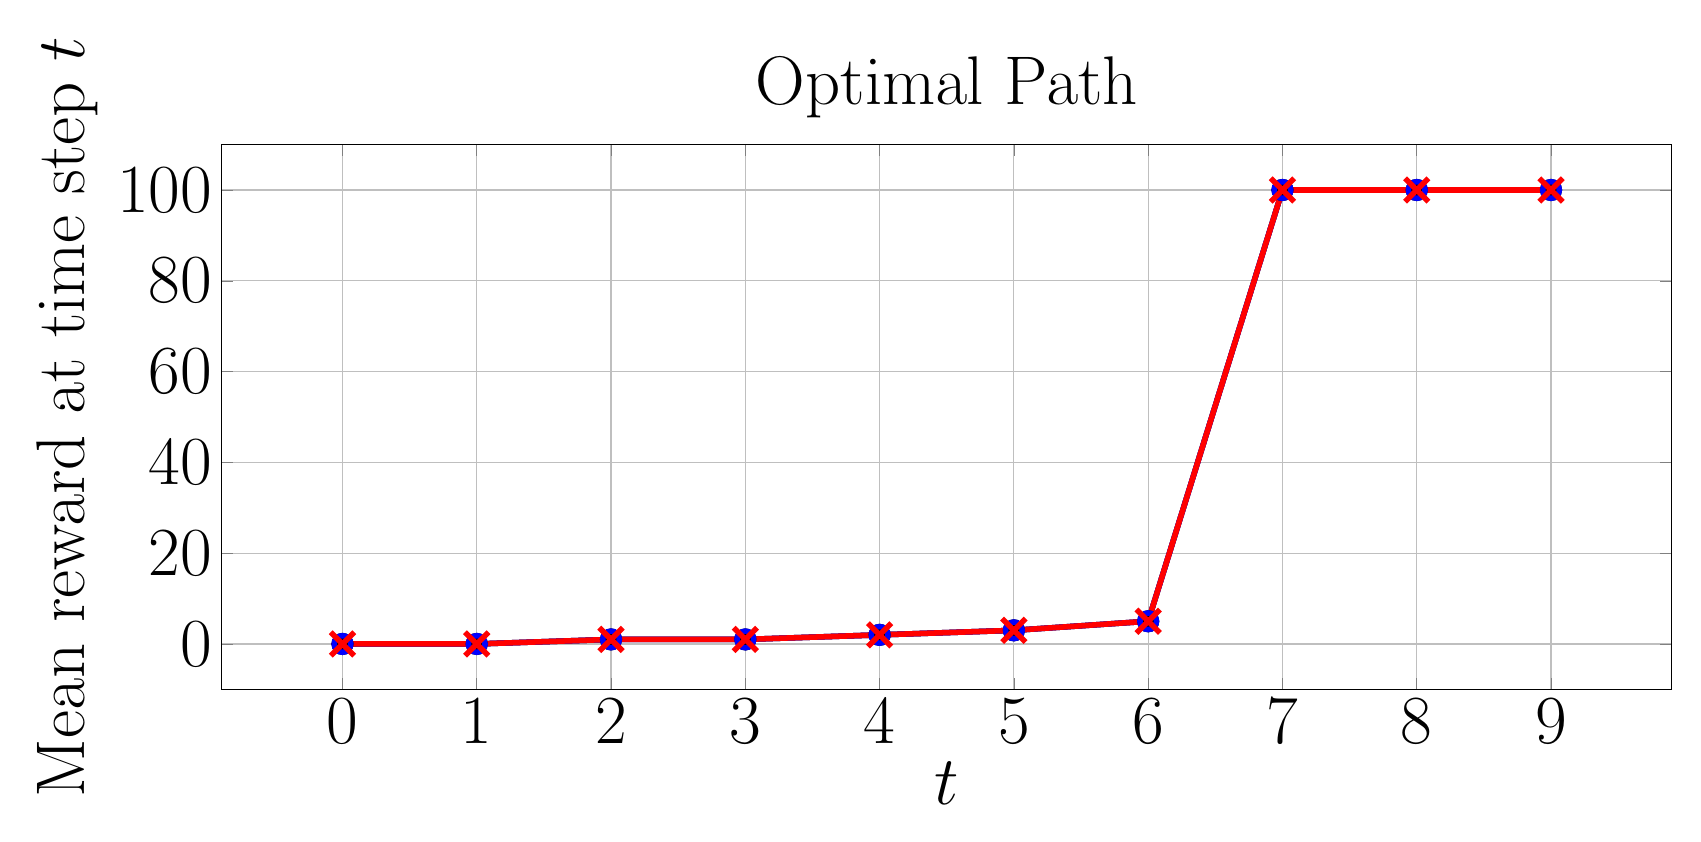
\begin{tikzpicture}
                \begin{axis}[
                    xlabel={$t$},
                    ylabel={Mean reward at time step $t$},
                    title={Optimal Path},
                    grid=both,
                    width=20cm, height=8.5cm,
                    every axis/.style={font=\Huge},
                    %
                ]
                \addplot[
                    color=black, %
                    mark=*, %
                    line width=2pt,
                    mark size=3pt,
                    error bars/.cd,
                    y dir=both, %
                    y explicit, %
                    error bar style={line width=1pt,solid},
                    error mark options={line width=1pt,mark size=4pt,rotate=90}
                ]
                coordinates {
                    (0, 0.0)  +- (0, 0.0)
                    (1, 0.0)  +- (0, 0.0) 
                    (2, 1.0)  +- (0, 0.0) 
                    (3, 1.0)  +- (0, 0.0)
                    (4, 2.0)  +- (0, 0.0)
                    (5, 3.0) +- (0, 0.0)
                    (6, 5.0) +- (0, 0.0)
                    (7, 100.0) +- (0, 0.0)
                    (8, 100.0) +- (0, 0.0)
                    (9, 100.0) +- (0, 0.0)
                };
                %
                \addplot[
                    color=blue, %
                    mark=o, %
                    line width=2pt,
                    mark size=3pt,
                    error bars/.cd,
                    y dir=both, %
                    y explicit, %
                    error bar style={line width=1pt,solid},
                    error mark options={line width=1pt,mark size=4pt,rotate=90}
                ]
                 coordinates {
                    (0, 0.0)  +- (0, 0.0)
                    (1, 0.0)  +- (0, 0.0) 
                    (2, 1.0)  +- (0, 0.0) 
                    (3, 1.0)  +- (0, 0.0)
                    (4, 2.0)  +- (0, 0.0)
                    (5, 3.0) +- (0, 0.0)
                    (6, 5.0) +- (0, 0.0)
                    (7, 100.0) +- (0, 0.0)
                    (8, 100.0) +- (0, 0.0)
                    (9, 100.0) +- (0, 0.0)
                };
                %
                \addplot[
                    color=red, %
                    mark=x, %
                    line width=2pt,
                    mark size=6pt,
                    error bars/.cd,
                    y dir=both, %
                    y explicit, %
                    error bar style={line width=1pt,solid},
                    error mark options={line width=1pt,mark size=4pt,rotate=90}
                ]
                coordinates {
                    (0, 0.0)  +- (0, 0.0)
                    (1, 0.0)  +- (0, 0.0) 
                    (2, 1.0)  +- (0, 0.0) 
                    (3, 1.0)  +- (0, 0.0)
                    (4, 2.0)  +- (0, 0.0)
                    (5, 3.0) +- (0, 0.0)
                    (6, 5.0) +- (0, 0.0)
                    (7, 100.0) +- (0, 0.0)
                    (8, 100.0) +- (0, 0.0)
                    (9, 100.0) +- (0, 0.0)
                };
                \end{axis}
            \end{tikzpicture}
         }
    }
    \hspace{1cm}
    \subfigure[\footnotesize Lowest cumulative reward: Interval CFMDP ($19$), Gumbel-max SCM ($-88$)]{%
         \resizebox{0.76\columnwidth}{!}{
            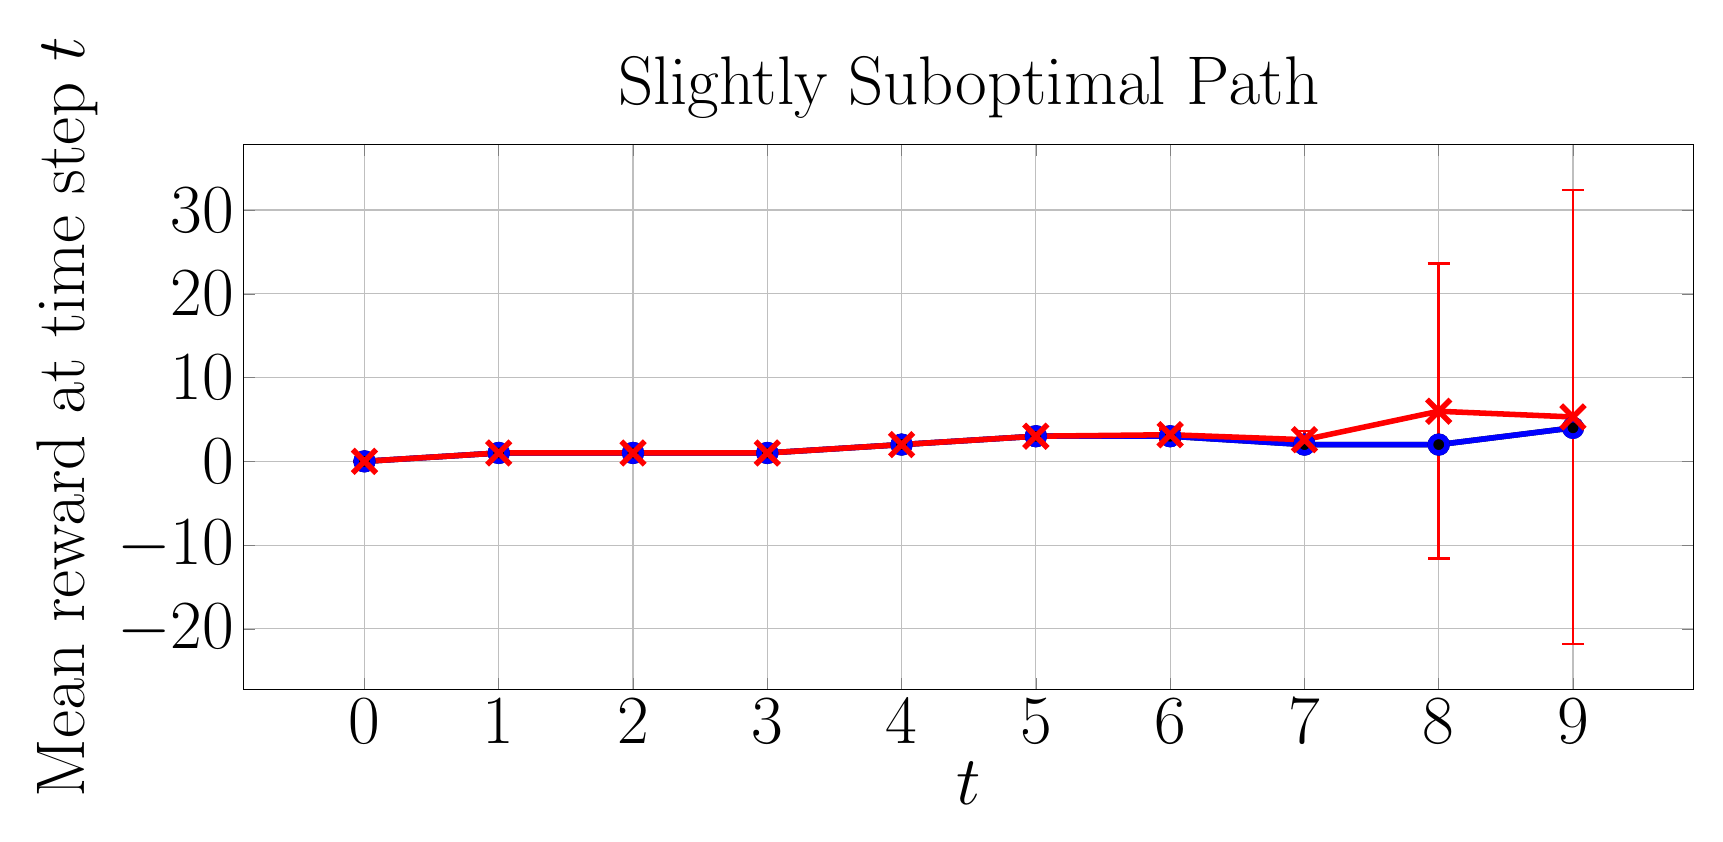
\begin{tikzpicture}
                \begin{axis}[
                    xlabel={$t$},
                    ylabel={Mean reward at time step $t$},
                    title={Slightly Suboptimal Path},
                    grid=both,
                    width=20cm, height=8.5cm,
                    every axis/.style={font=\Huge},
                    %
                ]
                \addplot[
                    color=black, %
                    mark=*, %
                    line width=2pt,
                    mark size=3pt,
                    error bars/.cd,
                    y dir=both, %
                    y explicit, %
                    error bar style={line width=1pt,solid},
                    error mark options={line width=1pt,mark size=4pt,rotate=90}
                ]
              coordinates {
                    (0, 0.0)  +- (0, 0.0)
                    (1, 1.0)  +- (0, 0.0) 
                    (2, 1.0)  +- (0, 0.0) 
                    (3, 1.0)  +- (0, 0.0)
                    (4, 2.0)  +- (0, 0.0)
                    (5, 3.0) +- (0, 0.0)
                    (6, 3.0) +- (0, 0.0)
                    (7, 2.0) +- (0, 0.0)
                    (8, 2.0) +- (0, 0.0)
                    (9, 4.0) +- (0, 0.0)
                };
                %
                \addplot[
                    color=blue, %
                    mark=o, %
                    line width=2pt,
                    mark size=3pt,
                    error bars/.cd,
                    y dir=both, %
                    y explicit, %
                    error bar style={line width=1pt,solid},
                    error mark options={line width=1pt,mark size=4pt,rotate=90}
                ]
              coordinates {
                    (0, 0.0)  +- (0, 0.0)
                    (1, 1.0)  +- (0, 0.0) 
                    (2, 1.0)  +- (0, 0.0) 
                    (3, 1.0)  +- (0, 0.0)
                    (4, 2.0)  +- (0, 0.0)
                    (5, 3.0) +- (0, 0.0)
                    (6, 3.0) +- (0, 0.0)
                    (7, 2.0) +- (0, 0.0)
                    (8, 2.0) +- (0, 0.0)
                    (9, 4.0) +- (0, 0.0)
                };
                %
                \addplot[
                    color=red, %
                    mark=x, %
                    line width=2pt,
                    mark size=6pt,
                    error bars/.cd,
                    y dir=both, %
                    y explicit, %
                    error bar style={line width=1pt,solid},
                    error mark options={line width=1pt,mark size=4pt,rotate=90}
                ]
                coordinates {
                    (0, 0.0)  +- (0, 0.0)
                    (1, 1.0)  +- (0, 0.0) 
                    (2, 1.0)  +- (0, 0.0) 
                    (3, 1.0)  +- (0, 0.0)
                    (4, 2.0)  += (0, 0.0)
                    (5, 3.0)  += (0, 0.0)
                    (6, 3.17847) += (0, 0.62606746) -= (0, 0.62606746)
                    (7, 2.5832885) += (0, 1.04598233) -= (0, 1.04598233)
                    (8, 5.978909) += (0, 17.60137623) -= (0, 17.60137623)
                    (9, 5.297059) += (0, 27.09227512) -= (0, 27.09227512)
                };
                \end{axis}
            \end{tikzpicture}
         }
    }\\[-1.5pt]
    \subfigure[\footnotesize Lowest cumulative reward: Interval CFMDP ($14$), Gumbel-max SCM ($-598$)]{%
         \resizebox{0.76\columnwidth}{!}{
             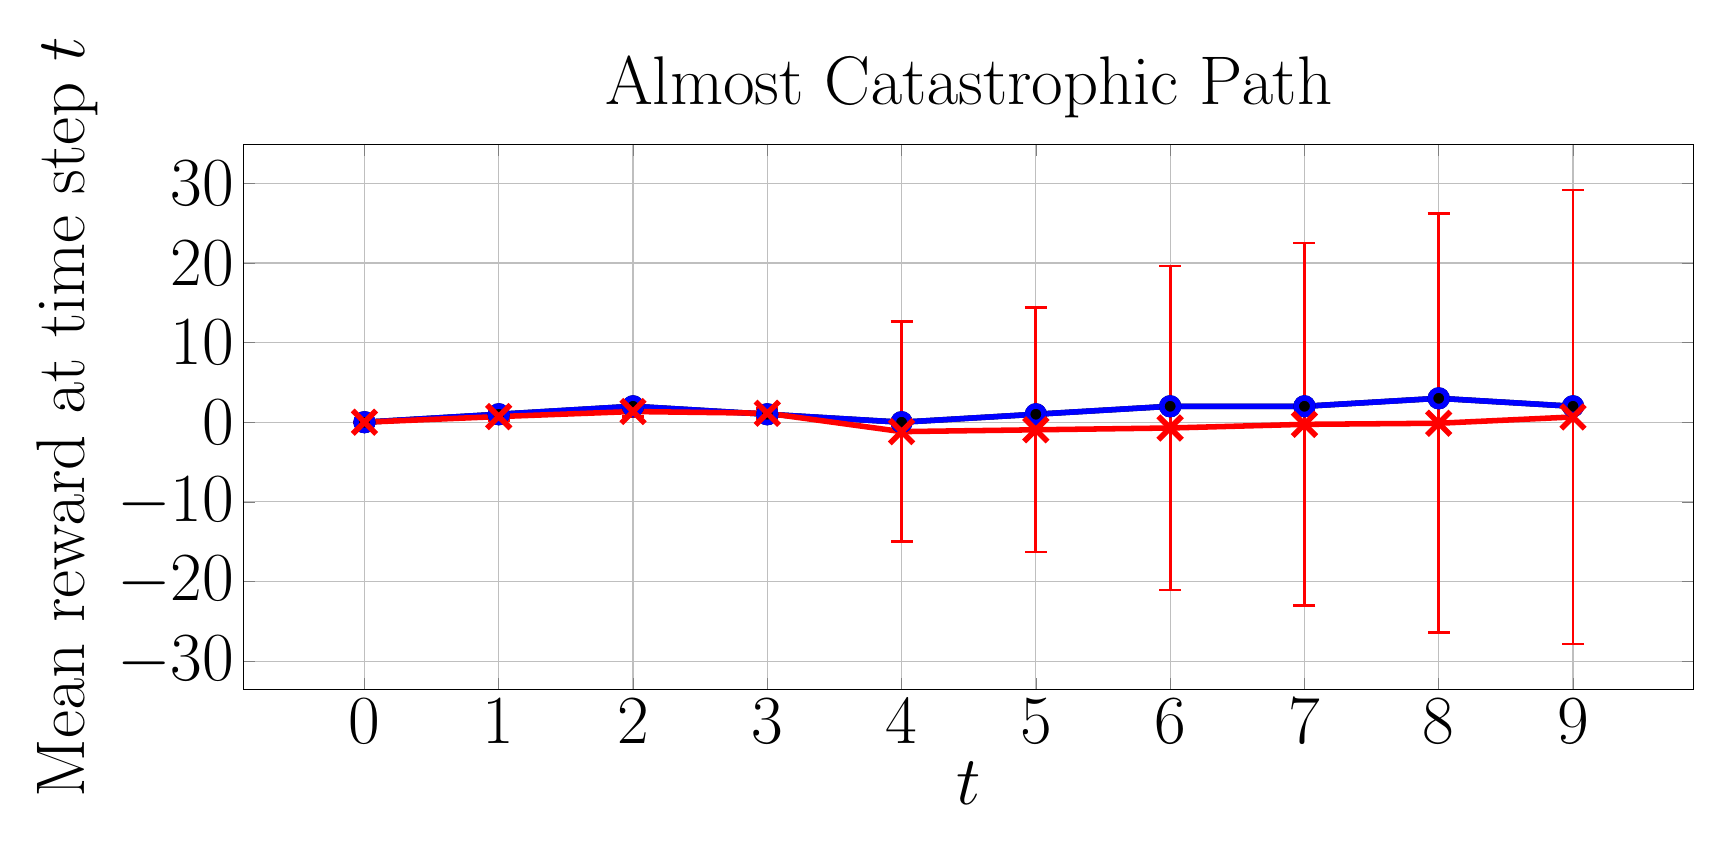
\begin{tikzpicture}
                \begin{axis}[
                    xlabel={$t$},
                    ylabel={Mean reward at time step $t$},
                    title={Almost Catastrophic Path},
                    grid=both,
                    width=20cm, height=8.5cm,
                    every axis/.style={font=\Huge},
                    %
                ]
                \addplot[
                    color=black, %
                    mark=*, %
                    line width=2pt,
                    mark size=3pt,
                    error bars/.cd,
                    y dir=both, %
                    y explicit, %
                    error bar style={line width=1pt,solid},
                    error mark options={line width=1pt,mark size=4pt,rotate=90}
                ]
                coordinates {
                    (0, 0.0)  +- (0, 0.0)
                    (1, 1.0)  +- (0, 0.0) 
                    (2, 2.0)  +- (0, 0.0) 
                    (3, 1.0)  +- (0, 0.0)
                    (4, 0.0)  +- (0, 0.0)
                    (5, 1.0) +- (0, 0.0)
                    (6, 2.0) +- (0, 0.0)
                    (7, 2.0) +- (0, 0.0)
                    (8, 3.0) +- (0, 0.0)
                    (9, 2.0) +- (0, 0.0)
                };
                %
                \addplot[
                    color=blue, %
                    mark=o, %
                    line width=2pt,
                    mark size=3pt,
                    error bars/.cd,
                    y dir=both, %
                    y explicit, %
                    error bar style={line width=1pt,solid},
                    error mark options={line width=1pt,mark size=4pt,rotate=90}
                ]
                coordinates {
                    (0, 0.0)  +- (0, 0.0)
                    (1, 1.0)  +- (0, 0.0) 
                    (2, 2.0)  +- (0, 0.0) 
                    (3, 1.0)  +- (0, 0.0)
                    (4, 0.0)  +- (0, 0.0)
                    (5, 1.0) +- (0, 0.0)
                    (6, 2.0) +- (0, 0.0)
                    (7, 2.0) +- (0, 0.0)
                    (8, 3.0) +- (0, 0.0)
                    (9, 2.0) +- (0, 0.0)
                };
                %
                \addplot[
                    color=red, %
                    mark=x, %
                    line width=2pt,
                    mark size=6pt,
                    error bars/.cd,
                    y dir=both, %
                    y explicit, %
                    error bar style={line width=1pt,solid},
                    error mark options={line width=1pt,mark size=4pt,rotate=90}
                ]
                coordinates {
                    (0, 0.0)  +- (0, 0.0)
                    (1, 0.7065655)  +- (0, 0.4553358) 
                    (2, 1.341673)  +- (0, 0.67091621) 
                    (3, 1.122926)  +- (0, 0.61281824)
                    (4, -1.1821935)  +- (0, 13.82444042)
                    (5, -0.952399)  +- (0, 15.35195457)
                    (6, -0.72672) +- (0, 20.33508414)
                    (7, -0.268983) +- (0, 22.77861454)
                    (8, -0.1310835) +- (0, 26.31013314)
                    (9, 0.65806) +- (0, 28.50670214)
                };
                %
            %
            %
            %
            %
            %
            %
            %
            %
            %
            %
            %
            %
            %
            %
            %
            %
            %
            %
                \end{axis}
            \end{tikzpicture}
         }
    }
    \hspace{1cm}
    \subfigure[\footnotesize Lowest cumulative reward: Interval CFMDP ($-698$), Gumbel-max SCM ($-698$)]{%
         \resizebox{0.76\columnwidth}{!}{
            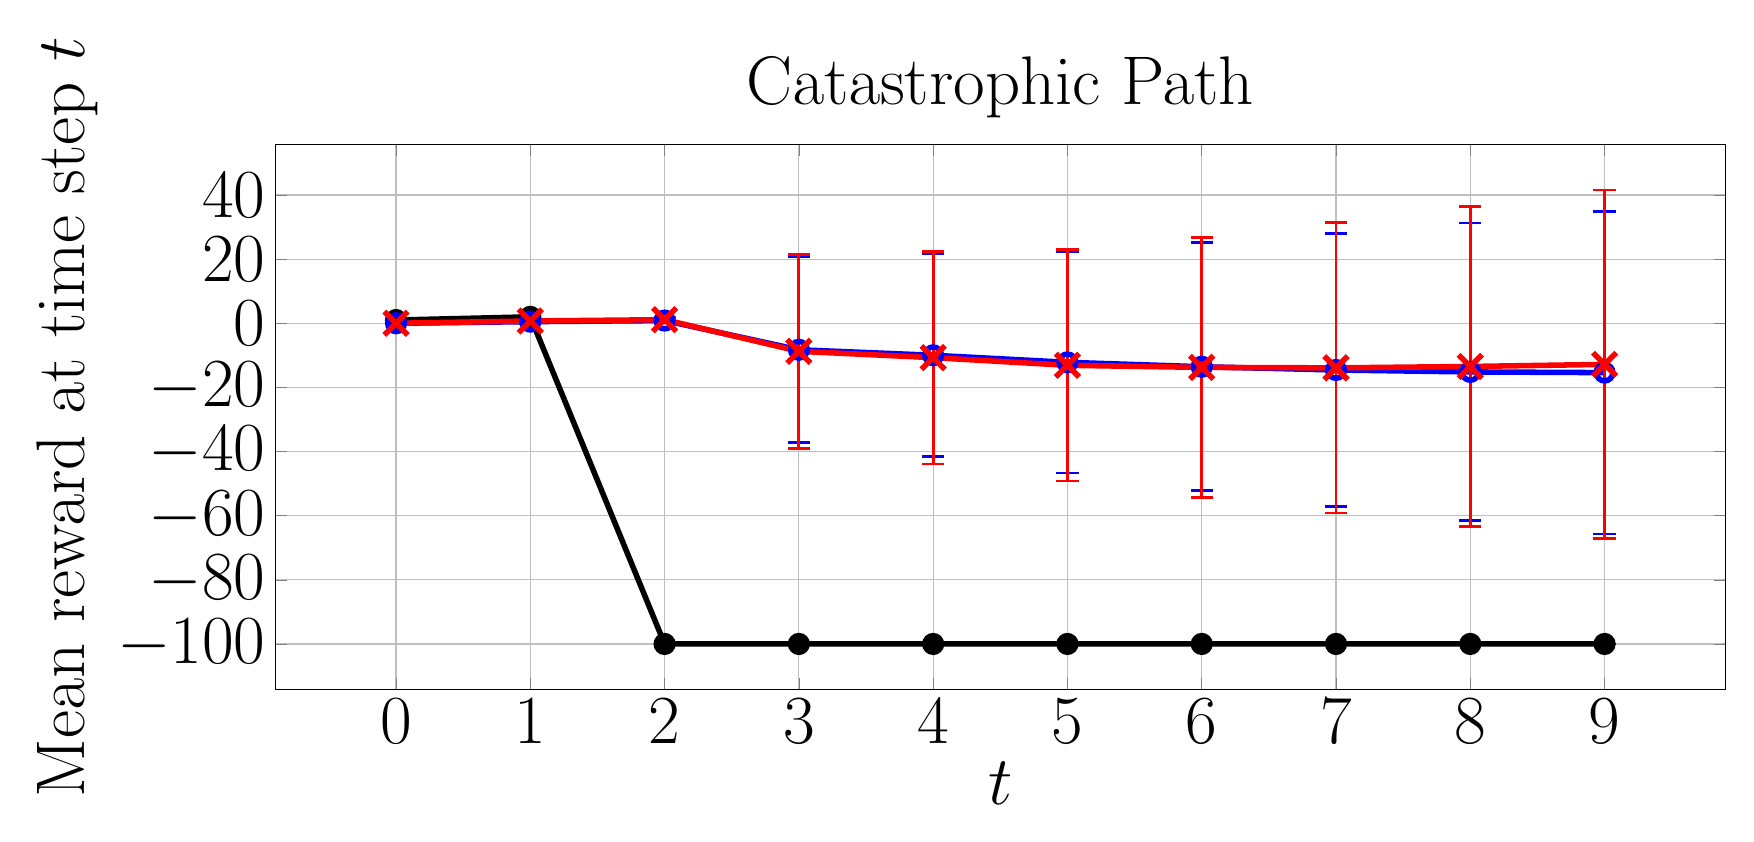
\begin{tikzpicture}
                \begin{axis}[
                    xlabel={$t$},
                    ylabel={Mean reward at time step $t$},
                    title={Catastrophic Path},
                    grid=both,
                    width=20cm, height=8.5cm,
                    every axis/.style={font=\Huge},
                    %
                ]
                \addplot[
                    color=black, %
                    mark=*, %
                    line width=2pt,
                    mark size=3pt,
                    error bars/.cd,
                    y dir=both, %
                    y explicit, %
                    error bar style={line width=1pt,solid},
                    error mark options={line width=1pt,mark size=4pt,rotate=90}
                ]
                coordinates {
                    (0, 1.0)  +- (0, 0.0)
                    (1, 2.0)  +- (0, 0.0) 
                    (2, -100.0)  +- (0, 0.0) 
                    (3, -100.0)  +- (0, 0.0)
                    (4, -100.0)  +- (0, 0.0)
                    (5, -100.0) +- (0, 0.0)
                    (6, -100.0) +- (0, 0.0)
                    (7, -100.0) +- (0, 0.0)
                    (8, -100.0) +- (0, 0.0)
                    (9, -100.0) +- (0, 0.0)
                };
                %
                \addplot[
                    color=blue, %
                    mark=o, %
                    line width=2pt,
                    mark size=3pt,
                    error bars/.cd,
                    y dir=both, %
                    y explicit, %
                    error bar style={line width=1pt,solid},
                    error mark options={line width=1pt,mark size=4pt,rotate=90}
                ]
                coordinates {
                    (0, 0.0)  +- (0, 0.0)
                    (1, 0.504814)  +- (0, 0.49997682) 
                    (2, 0.8439835)  +- (0, 0.76831917) 
                    (3, -8.2709165)  +- (0, 28.93656754)
                    (4, -9.981082)  +- (0, 31.66825363)
                    (5, -12.1776325) +- (0, 34.53463233)
                    (6, -13.556076) +- (0, 38.62845372)
                    (7, -14.574418) +- (0, 42.49603359)
                    (8, -15.1757075) +- (0, 46.41913968)
                    (9, -15.3900395) +- (0, 50.33563368)
                };
                %
                \addplot[
                    color=red, %
                    mark=x, %
                    line width=2pt,
                    mark size=6pt,
                    error bars/.cd,
                    y dir=both, %
                    y explicit, %
                    error bar style={line width=1pt,solid},
                    error mark options={line width=1pt,mark size=4pt,rotate=90}
                ]
                coordinates {
                    (0, 0.0)  +- (0, 0.0)
                    (1, 0.701873)  +- (0, 0.45743556) 
                    (2, 1.1227805)  +- (0, 0.73433129) 
                    (3, -8.7503255)  +- (0, 30.30257976)
                    (4, -10.722092)  +- (0, 33.17618589)
                    (5, -13.10721)  +- (0, 36.0648089)
                    (6, -13.7631645) +- (0, 40.56553451)
                    (7, -13.909043) +- (0, 45.23829402)
                    (8, -13.472517) +- (0, 49.96270296)
                    (9, -12.8278835) +- (0, 54.38618735)
                };
                %
            %
            %
            %
            %
            %
            %
            %
            %
            %
            %
            %
            %
            %
            %
            %
            %
            %
            %
                \end{axis}
            \end{tikzpicture}
         }
    }
    \caption{Average instant reward of CF paths induced by policies on GridWorld $p=0.4$.}
    \label{fig: reward p=0.4}
\end{figure*}

\subsection{Experimental Setup}
To compare policy performance, we measure the average rewards of counterfactual paths induced by our policy and the Gumbel-max policy by uniformly sampling $200$ counterfactual MDPs from the ICFMDP and generating $10,000$ counterfactual paths over each sampled CFMDP. \jl{Since the interval CFMDP depends on the observed path, we select $4$  paths of varying optimality to evaluate how the observed path impacts the performance of both policies: an optimal path, a slightly suboptimal path that could reach the optimal reward with a few changes, a catastrophic path that enters a catastrophic, terminal state with low reward, and an almost catastrophic path that was close to entering a catastrophic state.} When measuring the average probability bound widths and execution time needed to generate the ICFMDPs, we averaged over $20$ randomly generated observed paths
\footnote{Further training details are provided in Appendix \ref{app: training details}, and the code is provided at \href{https://github.com/ddv-lab/robust-cf-inference-in-MDPs}{https://github.com/ddv-lab/robust-cf-inference-in-MDPs}
%
%
.}.

\subsection{GridWorld}
\jl{The GridWorld MDP is a $4 \times 4$ grid where an agent must navigate from the top-left corner to the goal state in the bottom-right corner, avoiding a dangerous terminal state in the centre. At each time step, the agent can move up, down, left, or right, but there is a small probability (controlled by hyper-parameter $p$) of moving in an unintended direction. As the agent nears the goal, the reward for each state increases, culminating in a reward of $+100$ for reaching the goal. Entering the dangerous state results in a penalty of $-100$. We use two versions of GridWorld: a less stochastic version with $p=0.9$ (i.e., $90$\% chance of moving in the chosen direction) and a more stochastic version with $p=0.4$.}

\paragraph{GridWorld ($p=0.9$)}
When $p=0.9$, the counterfactual probability bounds are typically narrow (see Table \ref{tab:nonzero_probs} for average measurements). Consequently, as shown in Figure \ref{fig: reward p=0.9}, both policies are nearly identical and perform similarly well across the optimal, slightly suboptimal, and catastrophic paths.
%
However, for the almost catastrophic path, the interval CFMDP path is more conservative and follows the observed path more closely (as this is where the probability bounds are narrowest), which typically requires one additional step to reach the goal state than the Gumbel-max SCM policy.
%

\paragraph{GridWorld ($p=0.4$)}
\jl{When $p=0.4$, the GridWorld environment becomes more uncertain, increasing the risk of entering the dangerous state even if correct actions are chosen. Thus, as shown in Figure \ref{fig: reward p=0.4}, the interval CFMDP policy adopts a more conservative approach, avoiding deviation from the observed policy if it cannot guarantee higher counterfactual rewards (see the slightly suboptimal and almost catastrophic paths), whereas the Gumbel-max SCM is inconsistent: it can yield higher rewards, but also much lower rewards, reflected in the wide error bars.} For the catastrophic path, both policies must deviate from the observed path to achieve a higher reward and, in this case, perform similarly.
%
%
%
%
\subsection{Sepsis}
The Sepsis MDP \citep{oberst2019counterfactual} simulates trajectories of Sepsis patients. Each state consists of four vital signs (heart rate, blood pressure, oxygen concentration, and glucose levels), categorised as low, normal, or high.
and three treatments that can be toggled on/off at each time step (8 actions in total). Unlike \citet{oberst2019counterfactual}, we scale rewards based on the number of out-of-range vital signs, between $-1000$ (patient dies) and $1000$ (patient discharged). \jl{Like the GridWorld $p=0.4$ experiment, the Sepsis MDP is highly uncertain, as many states are equally likely to lead to optimal and poor outcomes. Thus, as shown in Figure \ref{fig: reward sepsis}, both policies follow the observed optimal and almost catastrophic paths to guarantee rewards are no worse than the observation.} However, improving the catastrophic path requires deviating from the observation. Here, the Gumbel-max SCM policy, on average, performs better than the interval CFMDP policy. But, since both policies have lower bounds clipped at $-1000$, neither policy reliably improves over the observation. In contrast, for the slightly suboptimal path, the interval CFMDP policy performs significantly better, shown by its higher lower bounds. 
Moreover, in these two cases, the worst-case counterfactual path generated by the interval CFMDP policy is better than that of the Gumbel-max SCM policy,
indicating its greater robustness.
%
\begin{figure*}
    \centering
     \resizebox{0.6\textwidth}{!}{
        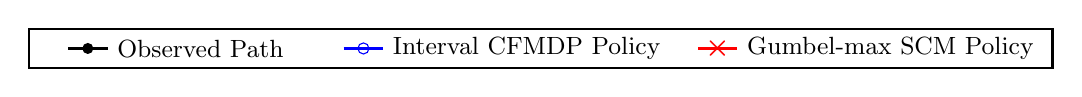
\begin{tikzpicture}[scale=1.0, every node/.style={scale=1.0}]
            \draw[thick, black] (-3, -0.25) rectangle (10, 0.25);
            %
            \draw[black, line width=1pt] (-2.5, 0.0) -- (-2,0.0);
            \fill[black] (-2.25,0.0) circle (2pt); %
            \node[right] at (-2,0.0) {\small Observed Path};
            
            %
            \draw[blue, line width=1pt] (1.0,0.0) -- (1.5,0.0);
            \node[draw=blue, circle, minimum size=4pt, inner sep=0pt] at (1.25,0.0) {}; %
            \node[right] at (1.5,0.0) {\small Interval CFMDP Policy};
            
            %
            \draw[red, line width=1pt] (5.5,0) -- (6,0);
            \node[red] at (5.75,0) {$\boldsymbol{\times}$}; %
            \node[right] at (6,0) {\small Gumbel-max SCM Policy};
        \end{tikzpicture}
    }\\
    \subfigure[\footnotesize Lowest cumulative reward: Interval CFMDP ($8000$), Gumbel-max SCM ($8000$)]{%
         \resizebox{0.76\columnwidth}{!}{
             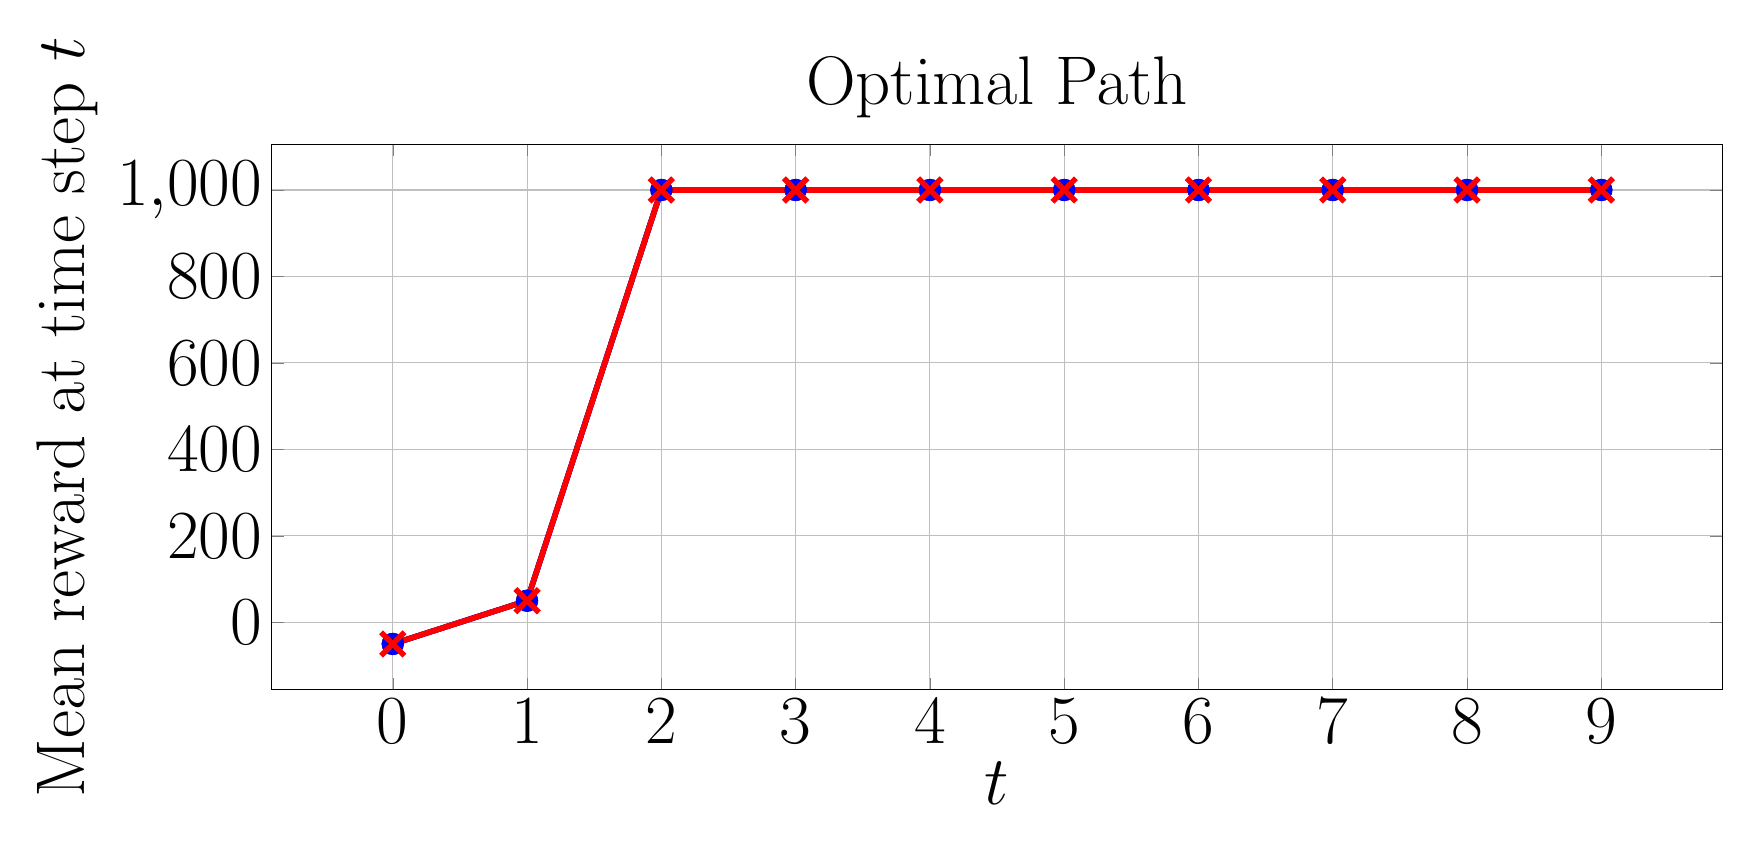
\begin{tikzpicture}
                \begin{axis}[
                    xlabel={$t$},
                    ylabel={Mean reward at time step $t$},
                    title={Optimal Path},
                    grid=both,
                    width=20cm, height=8.5cm,
                    every axis/.style={font=\Huge},
                    %
                ]
                \addplot[
                    color=black, %
                    mark=*, %
                    line width=2pt,
                    mark size=3pt,
                ]
                coordinates {
                    (0, -50.0)
                    (1, 50.0)
                    (2, 1000.0)
                    (3, 1000.0)
                    (4, 1000.0)
                    (5, 1000.0)
                    (6, 1000.0)
                    (7, 1000.0)
                    (8, 1000.0)
                    (9, 1000.0)
                };
                %
                \addplot[
                    color=blue, %
                    mark=o, %
                    line width=2pt,
                    mark size=3pt,
                    error bars/.cd,
                    y dir=both, %
                    y explicit, %
                    error bar style={line width=1pt,solid},
                    error mark options={line width=1pt,mark size=4pt,rotate=90}
                ]
                coordinates {
                    (0, -50.0)  +- (0, 0.0)
                    (1, 50.0)  +- (0, 0.0) 
                    (2, 1000.0)  +- (0, 0.0) 
                    (3, 1000.0)  +- (0, 0.0)
                    (4, 1000.0)  +- (0, 0.0)
                    (5, 1000.0) +- (0, 0.0)
                    (6, 1000.0) +- (0, 0.0)
                    (7, 1000.0) +- (0, 0.0)
                    (8, 1000.0) +- (0, 0.0)
                    (9, 1000.0) +- (0, 0.0)
                };
                %
                \addplot[
                    color=red, %
                    mark=x, %
                    line width=2pt,
                    mark size=6pt,
                    error bars/.cd,
                    y dir=both, %
                    y explicit, %
                    error bar style={line width=1pt,solid},
                    error mark options={line width=1pt,mark size=4pt,rotate=90}
                ]
                coordinates {
                    (0, -50.0)  +- (0, 0.0)
                    (1, 50.0)  +- (0, 0.0) 
                    (2, 1000.0)  +- (0, 0.0) 
                    (3, 1000.0)  +- (0, 0.0)
                    (4, 1000.0)  +- (0, 0.0)
                    (5, 1000.0) +- (0, 0.0)
                    (6, 1000.0) +- (0, 0.0)
                    (7, 1000.0) +- (0, 0.0)
                    (8, 1000.0) +- (0, 0.0)
                    (9, 1000.0) +- (0, 0.0)
                };
                %
                \end{axis}
            \end{tikzpicture}
         }
    }
    \hspace{1cm}
    \subfigure[\footnotesize Lowest cumulative reward: Interval CFMDP ($-5980$), Gumbel-max SCM ($-8000$)]{%
         \resizebox{0.76\columnwidth}{!}{
            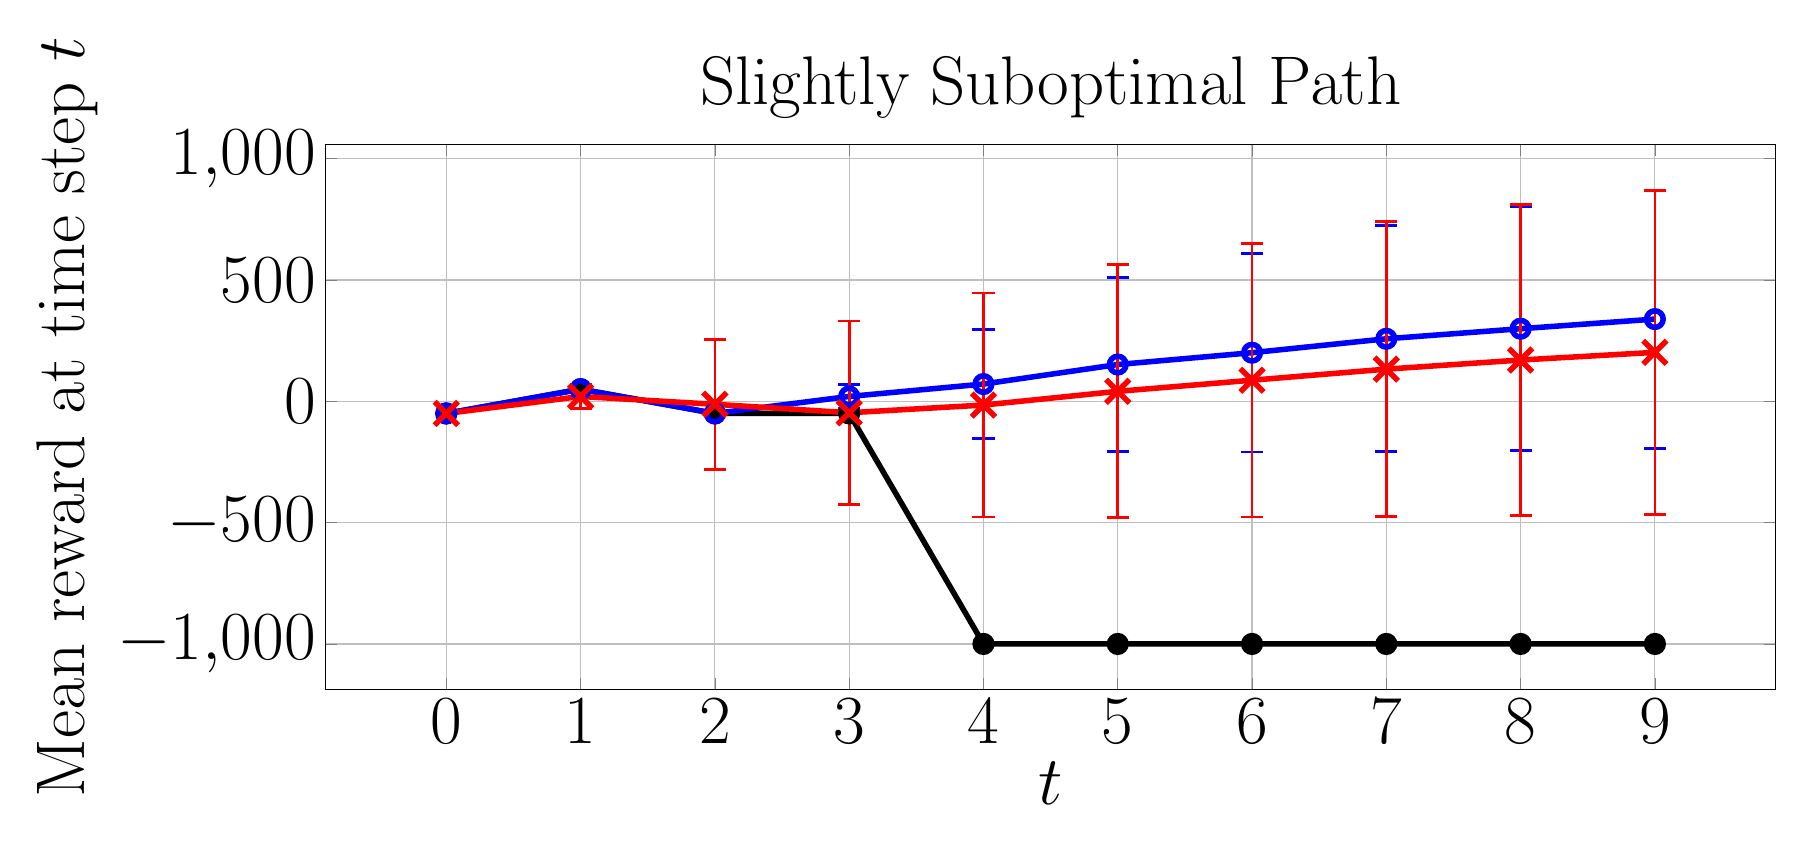
\begin{tikzpicture}
                \begin{axis}[
                    xlabel={$t$},
                    ylabel={Mean reward at time step $t$},
                    title={Slightly Suboptimal Path},
                    grid=both,
                    width=20cm, height=8.5cm,
                    every axis/.style={font=\Huge},
                    %
                ]
               \addplot[
                    color=black, %
                    mark=*, %
                    line width=2pt,
                    mark size=3pt,
                ]
                coordinates {
                    (0, -50.0)
                    (1, 50.0)
                    (2, -50.0)
                    (3, -50.0)
                    (4, -1000.0)
                    (5, -1000.0)
                    (6, -1000.0)
                    (7, -1000.0)
                    (8, -1000.0)
                    (9, -1000.0)
                };
                %
                \addplot[
                    color=blue, %
                    mark=o, %
                    line width=2pt,
                    mark size=3pt,
                    error bars/.cd,
                    y dir=both, %
                    y explicit, %
                    error bar style={line width=1pt,solid},
                    error mark options={line width=1pt,mark size=4pt,rotate=90}
                ]
                coordinates {
                    (0, -50.0)  +- (0, 0.0)
                    (1, 50.0)  +- (0, 0.0) 
                    (2, -50.0)  +- (0, 0.0) 
                    (3, 20.0631)  +- (0, 49.97539413)
                    (4, 71.206585)  +- (0, 226.02033693)
                    (5, 151.60797) +- (0, 359.23292559)
                    (6, 200.40593) +- (0, 408.86185176)
                    (7, 257.77948) +- (0, 466.10372804)
                    (8, 299.237465) +- (0, 501.82579506)
                    (9, 338.9129) +- (0, 532.06124996)
                };
                %
                \addplot[
                    color=red, %
                    mark=x, %
                    line width=2pt,
                    mark size=6pt,
                    error bars/.cd,
                    y dir=both, %
                    y explicit, %
                    error bar style={line width=1pt,solid},
                    error mark options={line width=1pt,mark size=4pt,rotate=90}
                ]
                coordinates {
                    (0, -50.0)  +- (0, 0.0)
                    (1, 20.00736)  +- (0, 49.99786741) 
                    (2, -12.282865)  +- (0, 267.598755) 
                    (3, -47.125995)  +- (0, 378.41755832)
                    (4, -15.381965)  +- (0, 461.77616558)
                    (5, 41.15459) +- (0, 521.53189262)
                    (6, 87.01595) +- (0, 564.22243126 )
                    (7, 132.62376) +- (0, 607.31338037)
                    (8, 170.168145) +- (0, 641.48013693)
                    (9, 201.813135) +- (0, 667.29441777)
                };
                %
                %
                %
                %
                %
                %
                %
                %
                %
                %
                %
                %
                %
                %
                %
                %
                %
                %
                %
                \end{axis}
            \end{tikzpicture}
         }
    }\\[-1.5pt]
    \subfigure[\footnotesize Lowest cumulative reward: Interval CFMDP ($100$), Gumbel-max SCM ($100$)]{%
         \resizebox{0.76\columnwidth}{!}{
             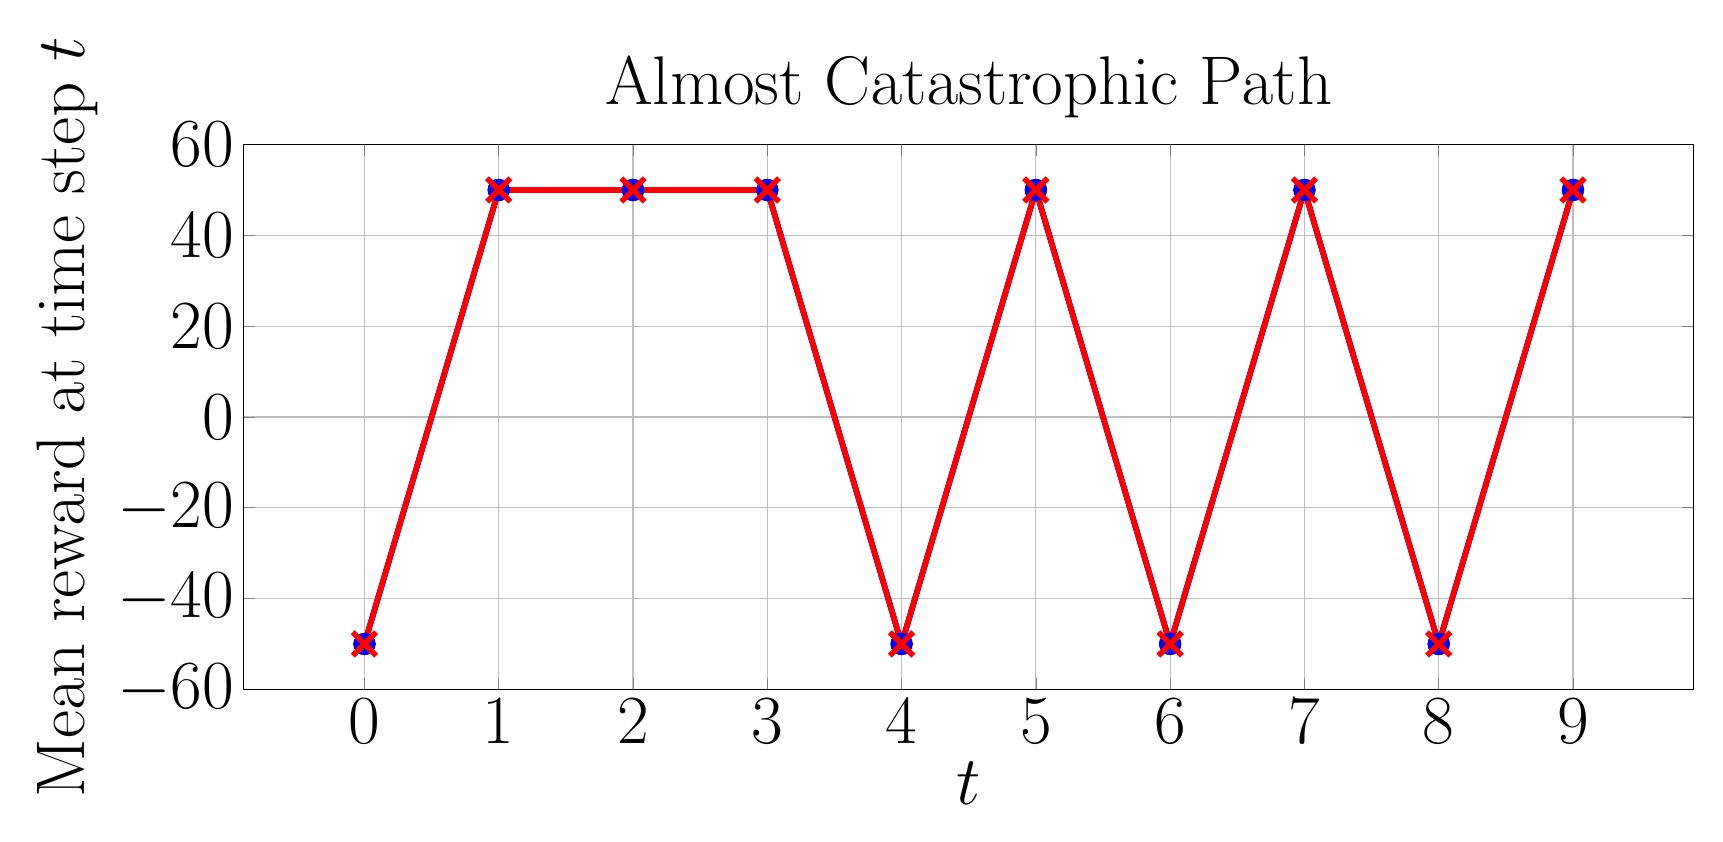
\begin{tikzpicture}
                \begin{axis}[
                    xlabel={$t$},
                    ylabel={Mean reward at time step $t$},
                    title={Almost Catastrophic Path},
                    grid=both,
                    every axis/.style={font=\Huge},
                    width=20cm, height=8.5cm,
                    %
                ]
               \addplot[
                    color=black, %
                    mark=*, %
                    line width=2pt,
                    mark size=3pt,
                ]
                coordinates {
                    (0, -50.0)
                    (1, 50.0)
                    (2, 50.0)
                    (3, 50.0)
                    (4, -50.0)
                    (5, 50.0)
                    (6, -50.0)
                    (7, 50.0)
                    (8, -50.0)
                    (9, 50.0)
                };
                %
                %
                \addplot[
                    color=blue, %
                    mark=o, %
                    line width=2pt,
                    mark size=3pt,
                    error bars/.cd,
                    y dir=both, %
                    y explicit, %
                    error bar style={line width=1pt,solid},
                    error mark options={line width=1pt,mark size=4pt,rotate=90}
                ]
                coordinates {
                    (0, -50.0)  +- (0, 0.0)
                    (1, 50.0)  +- (0, 0.0) 
                    (2, 50.0)  +- (0, 0.0) 
                    (3, 50.0)  +- (0, 0.0)
                    (4, -50.0)  +- (0, 0.0)
                    (5, 50.0) +- (0, 0.0)
                    (6, -50.0) +- (0, 0.0)
                    (7, 50.0) +- (0, 0.0)
                    (8, -50.0) +- (0, 0.0)
                    (9, 50.0) +- (0, 0.0)
                };
                %
                \addplot[
                    color=red, %
                    mark=x, %
                    line width=2pt,
                    mark size=6pt,
                    error bars/.cd,
                    y dir=both, %
                    y explicit, %
                    error bar style={line width=1pt,solid},
                    error mark options={line width=1pt,mark size=4pt,rotate=90}
                ]
                coordinates {
                    (0, -50.0)  +- (0, 0.0)
                    (1, 50.0)  +- (0, 0.0) 
                    (2, 50.0)  +- (0, 0.0) 
                    (3, 50.0)  +- (0, 0.0)
                    (4, -50.0)  +- (0, 0.0)
                    (5, 50.0) +- (0, 0.0)
                    (6, -50.0) +- (0, 0.0)
                    (7, 50.0) +- (0, 0.0)
                    (8, -50.0) +- (0, 0.0)
                    (9, 50.0) +- (0, 0.0)
                };
                %
                %
                %
                %
                %
                %
                %
                %
                %
                %
                %
                %
                %
                %
                %
                %
                %
                %
                %
                \end{axis}
            \end{tikzpicture}
         }
    }
    \hspace{1cm}
    \subfigure[\footnotesize Lowest cumulative reward: Interval CFMDP ($-7150$), Gumbel-max SCM ($-9050$)]{%
         \resizebox{0.76\columnwidth}{!}{
            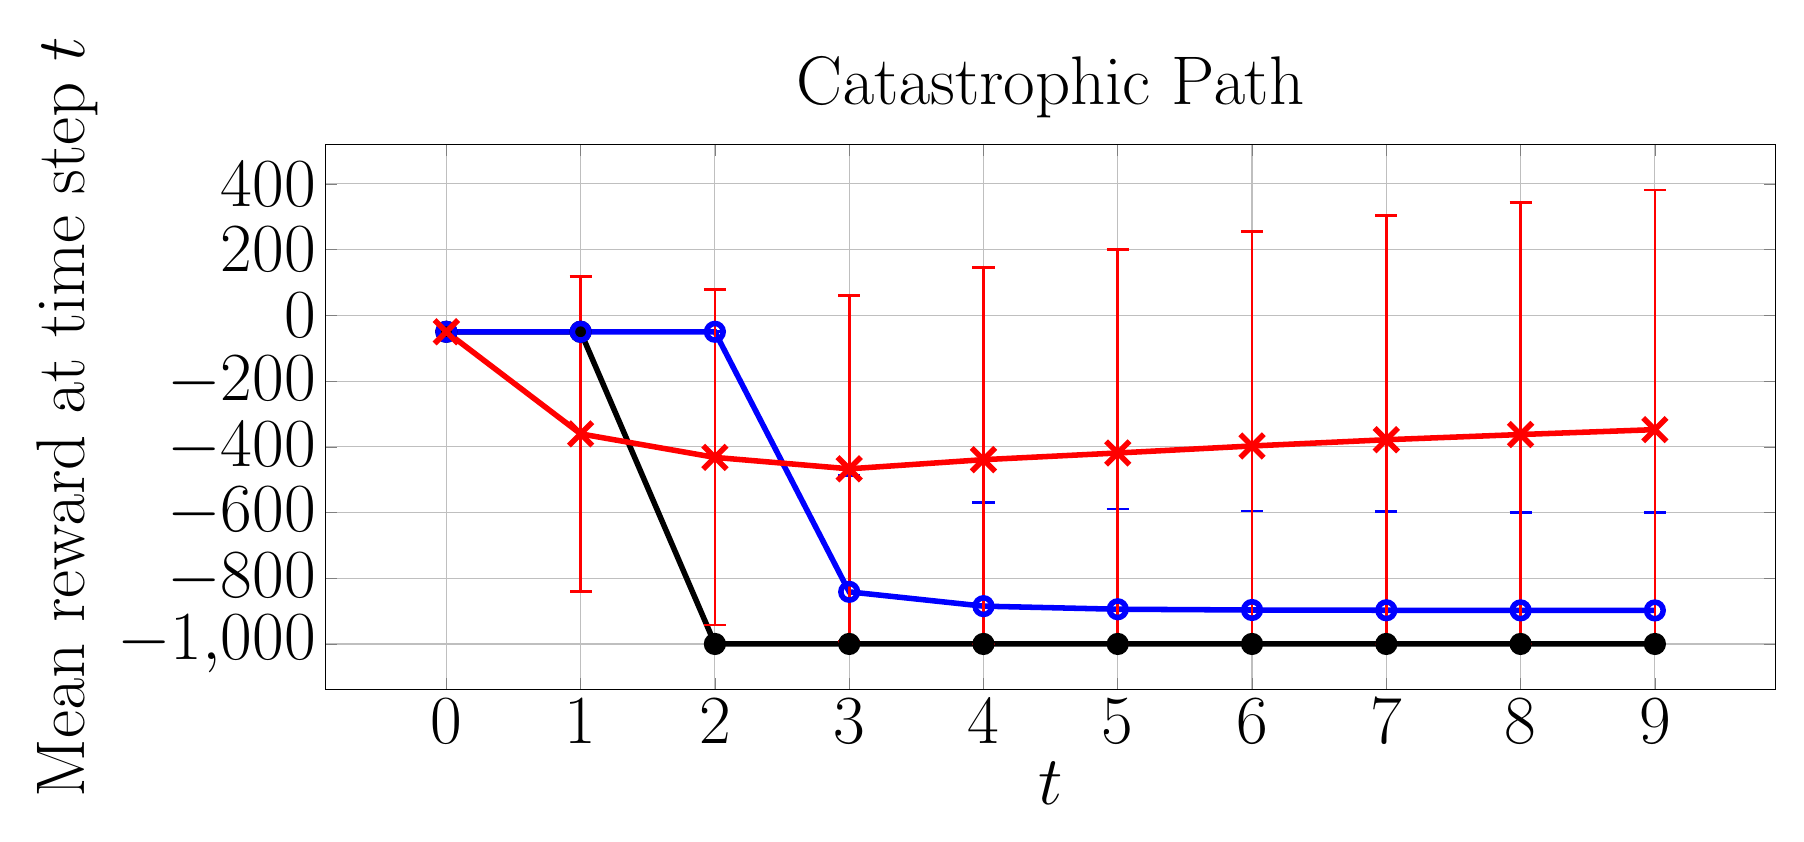
\begin{tikzpicture}
                \begin{axis}[
                    xlabel={$t$},
                    ylabel={Mean reward at time step $t$},
                    title={Catastrophic Path},
                    grid=both,
                    width=20cm, height=8.5cm,
                    every axis/.style={font=\Huge},
                    %
                ]
               \addplot[
                    color=black, %
                    mark=*, %
                    line width=2pt,
                    mark size=3pt,
                ]
                coordinates {
                    (0, -50.0)
                    (1, -50.0)
                    (2, -1000.0)
                    (3, -1000.0)
                    (4, -1000.0)
                    (5, -1000.0)
                    (6, -1000.0)
                    (7, -1000.0)
                    (8, -1000.0)
                    (9, -1000.0)
                };
                %
                %
                \addplot[
                    color=blue, %
                    mark=o, %
                    line width=2pt,
                    mark size=3pt,
                    error bars/.cd,
                    y dir=both, %
                    y explicit, %
                    error bar style={line width=1pt,solid},
                    error mark options={line width=1pt,mark size=4pt,rotate=90}
                ]
                coordinates {
                    (0, -50.0)  +- (0, 0.0)
                    (1, -50.0)  +- (0, 0.0) 
                    (2, -50.0)  +- (0, 0.0) 
                    (3, -841.440725)  += (0, 354.24605512) -= (0, 158.559275)
                    (4, -884.98225)  += (0, 315.37519669) -= (0, 115.01775)
                    (5, -894.330425) += (0, 304.88572805) -= (0, 105.669575)
                    (6, -896.696175) += (0, 301.19954514) -= (0, 103.303825)
                    (7, -897.4635) += (0, 299.61791279) -= (0, 102.5365)
                    (8, -897.77595) += (0, 298.80392585) -= (0, 102.22405)
                    (9, -897.942975) += (0, 298.32920557) -= (0, 102.057025)
                };
                %
                \addplot[
                    color=red, %
                    mark=x, %
                    line width=2pt,
                    mark size=6pt,
                    error bars/.cd,
                    y dir=both, %
                    y explicit, %
                    error bar style={line width=1pt,solid},
                    error mark options={line width=1pt,mark size=4pt,rotate=90}
                ]
            coordinates {
                    (0, -50.0)  +- (0, 0.0)
                    (1, -360.675265)  +- (0, 479.39812699) 
                    (2, -432.27629)  +- (0, 510.38620897) 
                    (3, -467.029545)  += (0, 526.36009628) -= (0, 526.36009628)
                    (4, -439.17429)  += (0, 583.96638919) -= (0, 560.82571)
                    (5, -418.82704) += (0, 618.43027478) -= (0, 581.17296)
                    (6, -397.464895) += (0, 652.67322574) -= (0, 602.535105)
                    (7, -378.49052) += (0, 682.85407033) -= (0, 621.50948)
                    (8, -362.654195) += (0, 707.01412023) -= (0, 637.345805)
                    (9, -347.737935) += (0, 729.29076479) -= (0, 652.262065)
                };
                %
                %
                %
                %
                %
                %
                %
                %
                %
                %
                %
                %
                %
                %
                %
                %
                %
                %
                %
                \end{axis}
            \end{tikzpicture}
         }
    }
    \caption{Average instant reward of CF paths induced by policies on Sepsis.}
    \label{fig: reward sepsis}
\end{figure*}

%
%
%
\subsection{Interval CFMDP Bounds}
%
%
Table \ref{tab:nonzero_probs} presents the mean counterfactual probability bound widths (excluding transitions where the upper bound is $0$) for each MDP, averaged over 20 observed paths. We compare the bounds under counterfactual stability (CS) and monotonicity (M) assumptions, CS alone, and no assumptions. This shows that the assumptions marginally reduce the bound widths, indicating the assumptions tighten the bounds without excluding too many causal models, as intended.
\renewcommand{\arraystretch}{1}

\begin{table}
\centering
\caption{Mean width of counterfactual probability bounds}
\resizebox{0.8\columnwidth}{!}{%
\begin{tabular}{|c|c|c|c|}
\hline
\multirow{2}{*}{\textbf{Environment}} & \multicolumn{3}{c|}{\textbf{Assumptions}} \\ \cline{2-4}
 & \textbf{CS + M} & \textbf{CS} & \textbf{None\tablefootnote{\jl{Equivalent to \citet{li2024probabilities}'s bounds (see Section \ref{sec: equivalence with Li}).}}} \\ \hline
\textbf{GridWorld} ($p=0.9$) & 0.0817 & 0.0977 & 0.100 \\ \hline
\textbf{GridWorld} ($p=0.4$) & 0.552  & 0.638  & 0.646 \\ \hline
\textbf{Sepsis} & 0.138 & 0.140 & 0.140 \\ \hline
\end{tabular}
}
\label{tab:nonzero_probs}
\end{table}


\subsection{Execution Times}
Table \ref{tab: times} compares the average time needed to generate the interval CFMDP vs.\ the Gumbel-max SCM CFMDP for 20 observations.
The GridWorld algorithms were run single-threaded, while the Sepsis experiments were run in parallel.
Generating the interval CFMDP is significantly faster as it uses exact analytical bounds, whereas the Gumbel-max CFMDP requires sampling from the Gumbel distribution to estimate counterfactual transition probabilities. \jl{Since constructing the counterfactual MDP models is the main bottleneck in both approaches, ours is more efficient overall and suitable for larger MDPs.}
\begin{table}
\centering
\caption{Mean execution time to generate CFMDPs}
\resizebox{0.99\columnwidth}{!}{%
\begin{tabular}{|c|c|c|}
\hline
\multirow{2}{*}{\textbf{Environment}} & \multicolumn{2}{c|}{\textbf{Mean Execution Time (s)}} \\ \cline{2-3} 
                                      & \textbf{Interval CFMDP} & \textbf{Gumbel-max CFMDP} \\ \hline
\textbf{GridWorld ($p=0.9$) }                  & 0.261                   & 56.1                      \\ \hline
\textbf{GridWorld ($p=0.4$)  }                 & 0.336                   & 54.5                      \\ \hline
\textbf{Sepsis}                                 & 688                     & 2940                      \\ \hline
\end{tabular}%
}
\label{tab: times}
\end{table}

\section{Conclusion}
In this work, we propose a simple yet effective approach, called SMILE, for graph few-shot learning with fewer tasks. Specifically, we introduce a novel dual-level mixup strategy, including within-task and across-task mixup, for enriching the diversity of nodes within each task and the diversity of tasks. Also, we incorporate the degree-based prior information to learn expressive node embeddings. Theoretically, we prove that SMILE effectively enhances the model's generalization performance. Empirically, we conduct extensive experiments on multiple benchmarks and the results suggest that SMILE significantly outperforms other baselines, including both in-domain and cross-domain few-shot settings.

\section{Acknowledgments}
% \footnotesize
This research was supported by the National Science Foundation under Grant OAC-2104023, OAC-2311875, OAC-2311876, OAC-2311878, OAC-2344717, and by the U.S. Department of Energy, Office of Science, Advanced Scientific Computing Research (ASCR), under contract DE-AC02-06CH11357.
This work used the Purdue Anvil CPU cluster through allocation CIS230308 and CIS240192 from the Advanced Cyberinfrastructure Coordination Ecosystem: Services \& Support (ACCESS) program.

% \bibliographystyle{IEEEtran}
\bibliographystyle{ACM-Reference-Format}
\bibliography{citations.bib}

% \balance
\end{document}
